\begin{quote}
  In order to make use of the Manhattan world assumption we must first
  discover the orientation of the Manhattan world with respect to the
  camera. This chapter focuses on estimating a 3D rotation that
  transforms the three cardinal Manhattan orientations onto the $x$,
  $y$, and $z$ axes. In contrast to much previous work, we seek to
  recover this rotation given a sequence of calibrated images, such as
  may be provided by a structure--from--motion or SLAM system. Where
  previous multiple--view approaches have focused on surface normal
  estimates derived from a reconstructed point cloud, we build upon
  ideas from single--view vanishing point detection and cast
  estimation in terms of photometric information. We develop a
  probabilistic model relating observed line segments to the 3D
  rotation we seek, and solve maximum--likelihood inference using an
  Expectation--Maximisation algorithm. Our likelihoods are derived
  from principled error models, and estimation is performed as a
  single optimisation.  We show that our approach substantially
  out--performs a state--of--the--art approach based on surface
  normals, while providing much greater robustness than single--view
  vanishing point estimation.\footnotemark
\end{quote}

\footnotetext{This work was published in part in:

{ \setlength{\parindent}{0pt} 
  \textit{Flint, Mei, Murray, and Reid,} ``Growing Semantically
  Meaningful Models For Visual SLAM'', in \textit{Proceedings of the
    2010 Conference on Computer Vision and Pattern
    Recognition}\cite{Flint10cvpr} 
} 
}

\section{Introduction}

Many man--made environments contain numerous surfaces oriented in
three mutually orthogonal directions. In order to leverage the special
structure of these Manhattan scenes we must identify these three
canonical directions. Since these directions are assumed to be
orthogonal to one another, identifying them is equivalent to finding a
3--dimensional rotation $\SceneR$ that maps them onto the $x$, $y$,
and $z$ axes.

We assume that an estimate of the camera pose for each frame is
available, such as might be provided by a structure--from--motion
system. We will not use any point cloud generated from
structure--from--motion in this chapter. We assume that the provided
camera poses are measured in a fixed but arbitrary coordinate
frame. Determining $\SceneR$ in the context of a single
image is equivalent to detecting vanishing points since three
vanishing points and a calibrated camera are sufficient to recover
$\SceneR$. However, in the multiple view context it makes sense to
estimate $\SceneR$ jointly using all available information, rather
than to merge single--view estimates post--hoc. One view of the
contribution of this chapter is therefore as a generalisation of
vanishing point detection to multiple calibrated views.

We estimate $\SceneR$ using the assumption that a significant number
of the observed line segments correspond to one of three Manhattan
orientations. We present a graphical model relating line segments to
$\SceneR$, then we present an Expectation--Maximisation algorithm for
inference within this model. Our likelihoods are derived from a
well--defined model of image formation, and we optimise jointly with
respect to all line segments in all views in a single
optimisation. Our approach parallels ideas presented in the
context of single--view vanishing point detection, particularly those
of Andrew Zisserman \cite{Hartley04} and Frank Dellaert
\cite{Schindler2004}. Our contribution is a principled way to
incorporate multiple calibrated views into a single optimisation, and
an empirical demonstration that doing so significantly out--performs
both single--view vanishing point estimation and
surface--normal--based estimators.

\section{Background}

Vanishing point detection has a long history in the computer vision
literature, beginning with the seminal work of
Barnard \etal \cite{BARNARD1983}. In this section we survey key
contributions within this literature and discuss their relationship to
our work.

\subsection{Single View Approaches}

Several approaches to single--image vanishing point detection have
been proposed in the literature
\cite{BARNARD1983,Zhang02,Shufelt99}. Common among all such approaches
is the use of line segments as the fundamental observation from which
inference is performed. The vanishing points under consideration are
assumed to generate several associated line segments, all of which
meet at the vanishing point (modulo measurement errors). The
estimation of vanishing points is approached in various ways. The
classic approach due to Barnard \cite{BARNARD1983} was to project
images onto the Gaussian sphere and use the Hough transform to
identify vanishing points. Several authors have proposed similar
voting schemes under different parametrisations of the accumulator
space that improve statistical robustness.

Shufelt \cite{Shufelt99} introduced explicit error models for observed
line segments, but retained the voting--based estimation
strategy. Hartley and Zisserman \cite{Hartley04} first proposed a
generative model relating vanishing point to line segments and cast
maximum likelihood estimation as a non--linear estimation problem. We
make similar modelling assumptions in the present
work. Kanatani \cite{Kanatani93} minimised the algebraic deviation of
vanishing points from observed line segments, which leads to an
efficient linear least--squares solution at the cost of a less precise
error model. Schinder and Dellaert \cite{Schindler2004} laid out an
integrated Bayesian approach to the estimation of multiple vanishing
points.

The approaches discussed thus far estimate vanishing points
independently, using K--means clustering or the expectation
maximisation algorithm to resolve the assignment of line segments to
vanishing points. Coughlan and Yuille \cite{Coughlan99} observed that
under the Manhattan world assumption the three cardinal vanishing
points are mutually orthogonal and hence their locations in the image
plane are highly correlated. Rather than estimating three independent
vanishing points, the authors cast the estimation problems in terms of
Euler angles corresponding to $\SceneR$, resulting in a three--DoF
estimation problem in place of the 6 for independent vanishing point
estimation. Koseck\`{a} and Zhang \cite{Zhang02} showed that the
Manhattan world assumption can be exploited even in the case of an
uncalibrated camera. Their approach used a prior on camera intrinsics
to condition the estimation process, though the estimation of three
vanishing points was not explicitly coupled after this stage.

Denis \etal \cite{Denis2008} took this a step further by
exploiting a prior on the rotation $\SceneR$ learned from training
data. Whereas Coughlan and Yuille used a discretisation of the space
of rotations to identify $\SceneR$, they showed how to exploit the
Manhattan world assumption under the more principled
Expectation--Maximisation approach of Schindler and Dellaert
\cite{Schindler2004}. The M--step in their approach is a non--linear
optimisation over rotations, leveraging the maximum likelihood
reprojection error of Hartley and Zisserman\cite{Hartley04}.

\changedsinceviva{
Sinha \etal \cite{Sinha2008} show how vanishing points in different
views can be optimised jointly with structure and motion inside a
single bundle adjustment. Their approach fixes the
line/vanishing--point associations using multi--hypothesis RANSAC in
individual views. Structure, motion, and vanishing directions are then
optimised jointly while holding the data associations fixed. Our approach
differs from theirs in that (1) we optimise the data association
variables linking lines to vanishing points jointly with the vanishing
point locations; and (2) we do not refine structure and motion using
the vanishing points.
}

Mirzaei and Roumeliotis \cite{Mirzaei2011} showed that
minimising the algebraic error for three mutually orthogonal vanishing
points can be solved globally using a polynomial solver. Their
approach assumes the algebraic error; it is not clear whether the
reprojection error leads to a likelihood that is amenable to a
polynomial solution.

\changedsinceviva{
Bazin \etal \cite{Bazin2012} recently proposed a novel
globally--optimal vanishing point algorithm based on
branch--and--bound. They search over partitions of the observed
line segments, constrained by the requirement that each partition must
be consistent with some vanishing point to a tolerance $\tau$. This
approach is attractive because it is guaranteed to find the global
optimum. The authors optimise an objective function based on the
number of consistent line segments, whereas most previous approaches
optimise a log--likelihood.
}

\subsection{Multiple View Approaches}

The literature concerning vanishing point estimation from multiple
views is sparse, and generally involves non--photometric approaches to
recover $\SceneR$. Furukawa and Curless \cite{Furukawa09} use
multiple--view stereo to recover a dense point cloud, then estimate
$\SceneR$ by clustering surface normals on the unit hemisphere. Werner
and Zisserman \cite{Werner2002} identify vanishing points
independently in several uncalibrated views, then resolve associations
between views using a combinatorial search.

\section{Overview of Proposed Approach}

Reliable vanishing point detection from single images is fundamentally
challenging in environments in which axis--oriented edges are rare, or
in which one or two cardinal orientations have very few associated
edges. Both scenarios are common in video sequences of indoor
environments since the camera often views only a small portion of the
scene. On the other hand, obtaining a dense reconstruction is a
complex and computationally expensive pre--requisite for a
three--parameter estimation problem. Furthermore, the point cloud
provided by on--line structure--from--motion is too sparse to obtain
accurate surface normal estimates.

We overcome these difficulties by reasoning in terms of line
segments and integrating observations from many frames into the
estimation. Since $\SceneR$ is fixed for all frames it makes sense to
leverage all available data during estimation. Whereas previous
approaches often estimate vanishing points as a precursor to
reconstructing camera poses \cite{Zhang02,Werner2002}, we prefer to rely
on the structure--from--motion system to provide camera poses,
then recover vanishing points afterwards. Under this problem setup we
can relate line segments in all views directly to $\SceneR$ and
therefore incorporate all available evidence into a joint
estimation. We show that this is both computationally efficient and
avoids the fragile single--view estimation scenario.

\changedsinceviva{
The structure--from--motion system we have chosen to work with is the
parallel tracking and mapping (PTAM) approach of Klein and Murray
\cite{Klein07}. This approach is suitable for online experiments,
although this comes at the cost of reduced accuracy compared to global
bundle adjustment. Importantly, PTAM can encounter scale and
orientation drift, so the maps it builds may not be perfectly
metric. While our results with this system are promising, we do notice
small vanishing point inconsistencies between frames, which can lead
to errors in our reconstructions. When operating offline, this could
be alleviated by running global bundle adjustment prior to executing
our system.
}

\section{Generative Model}

\begin{figure}[tb]
  \centering
  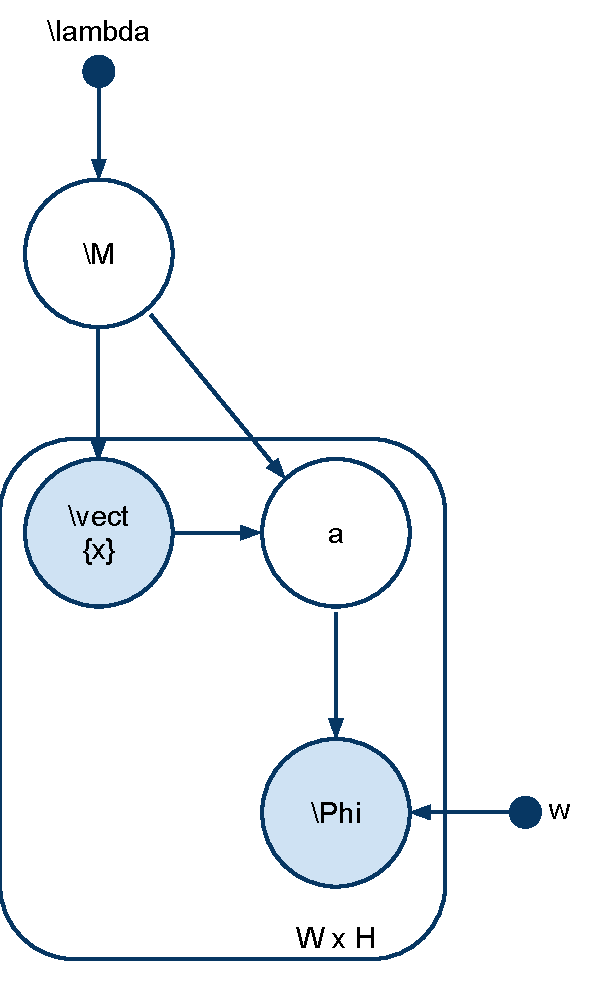
\includegraphics[width=0.5\textwidth]{graphical-model}
  \caption{A graphical model relating line segments to vanishing
    points.}
  \label{fig:R-graphical}
\end{figure}

\begin{figure}[tb]
  \centering
  \subfloat[Error model for line observations.]{
    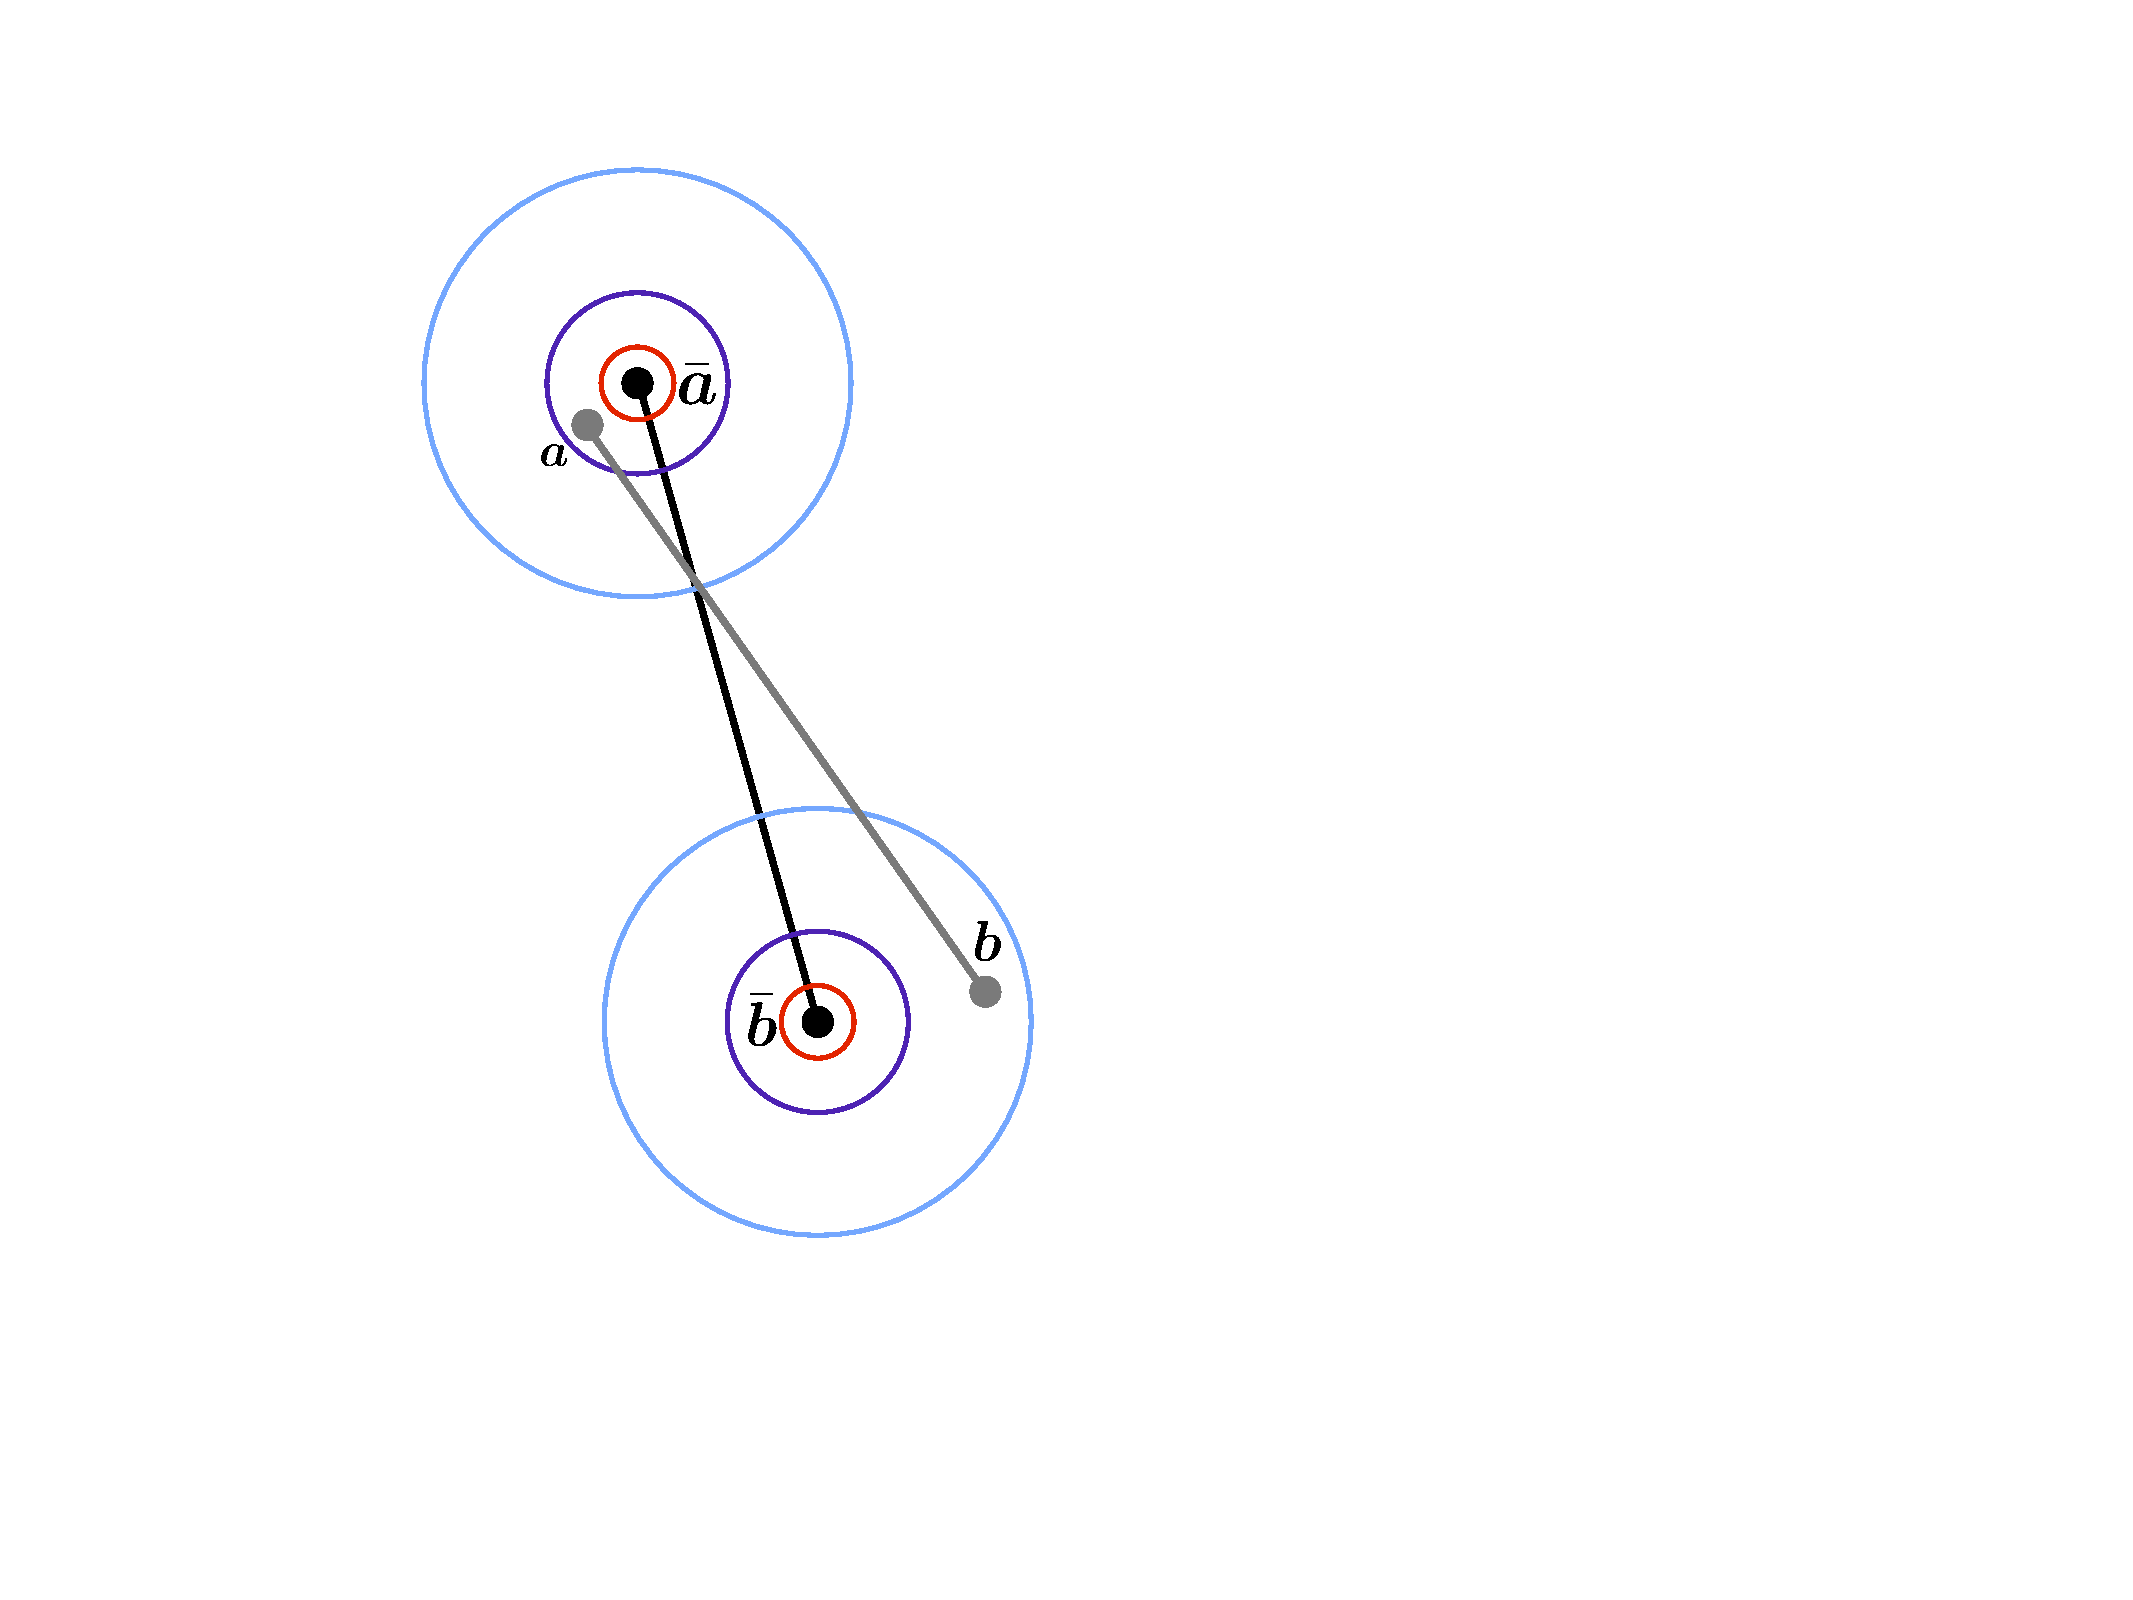
\includegraphics[width=0.4\textwidth]{error-model}
  }
  \qquad
  \subfloat[The reprojection error, $d$.]{
    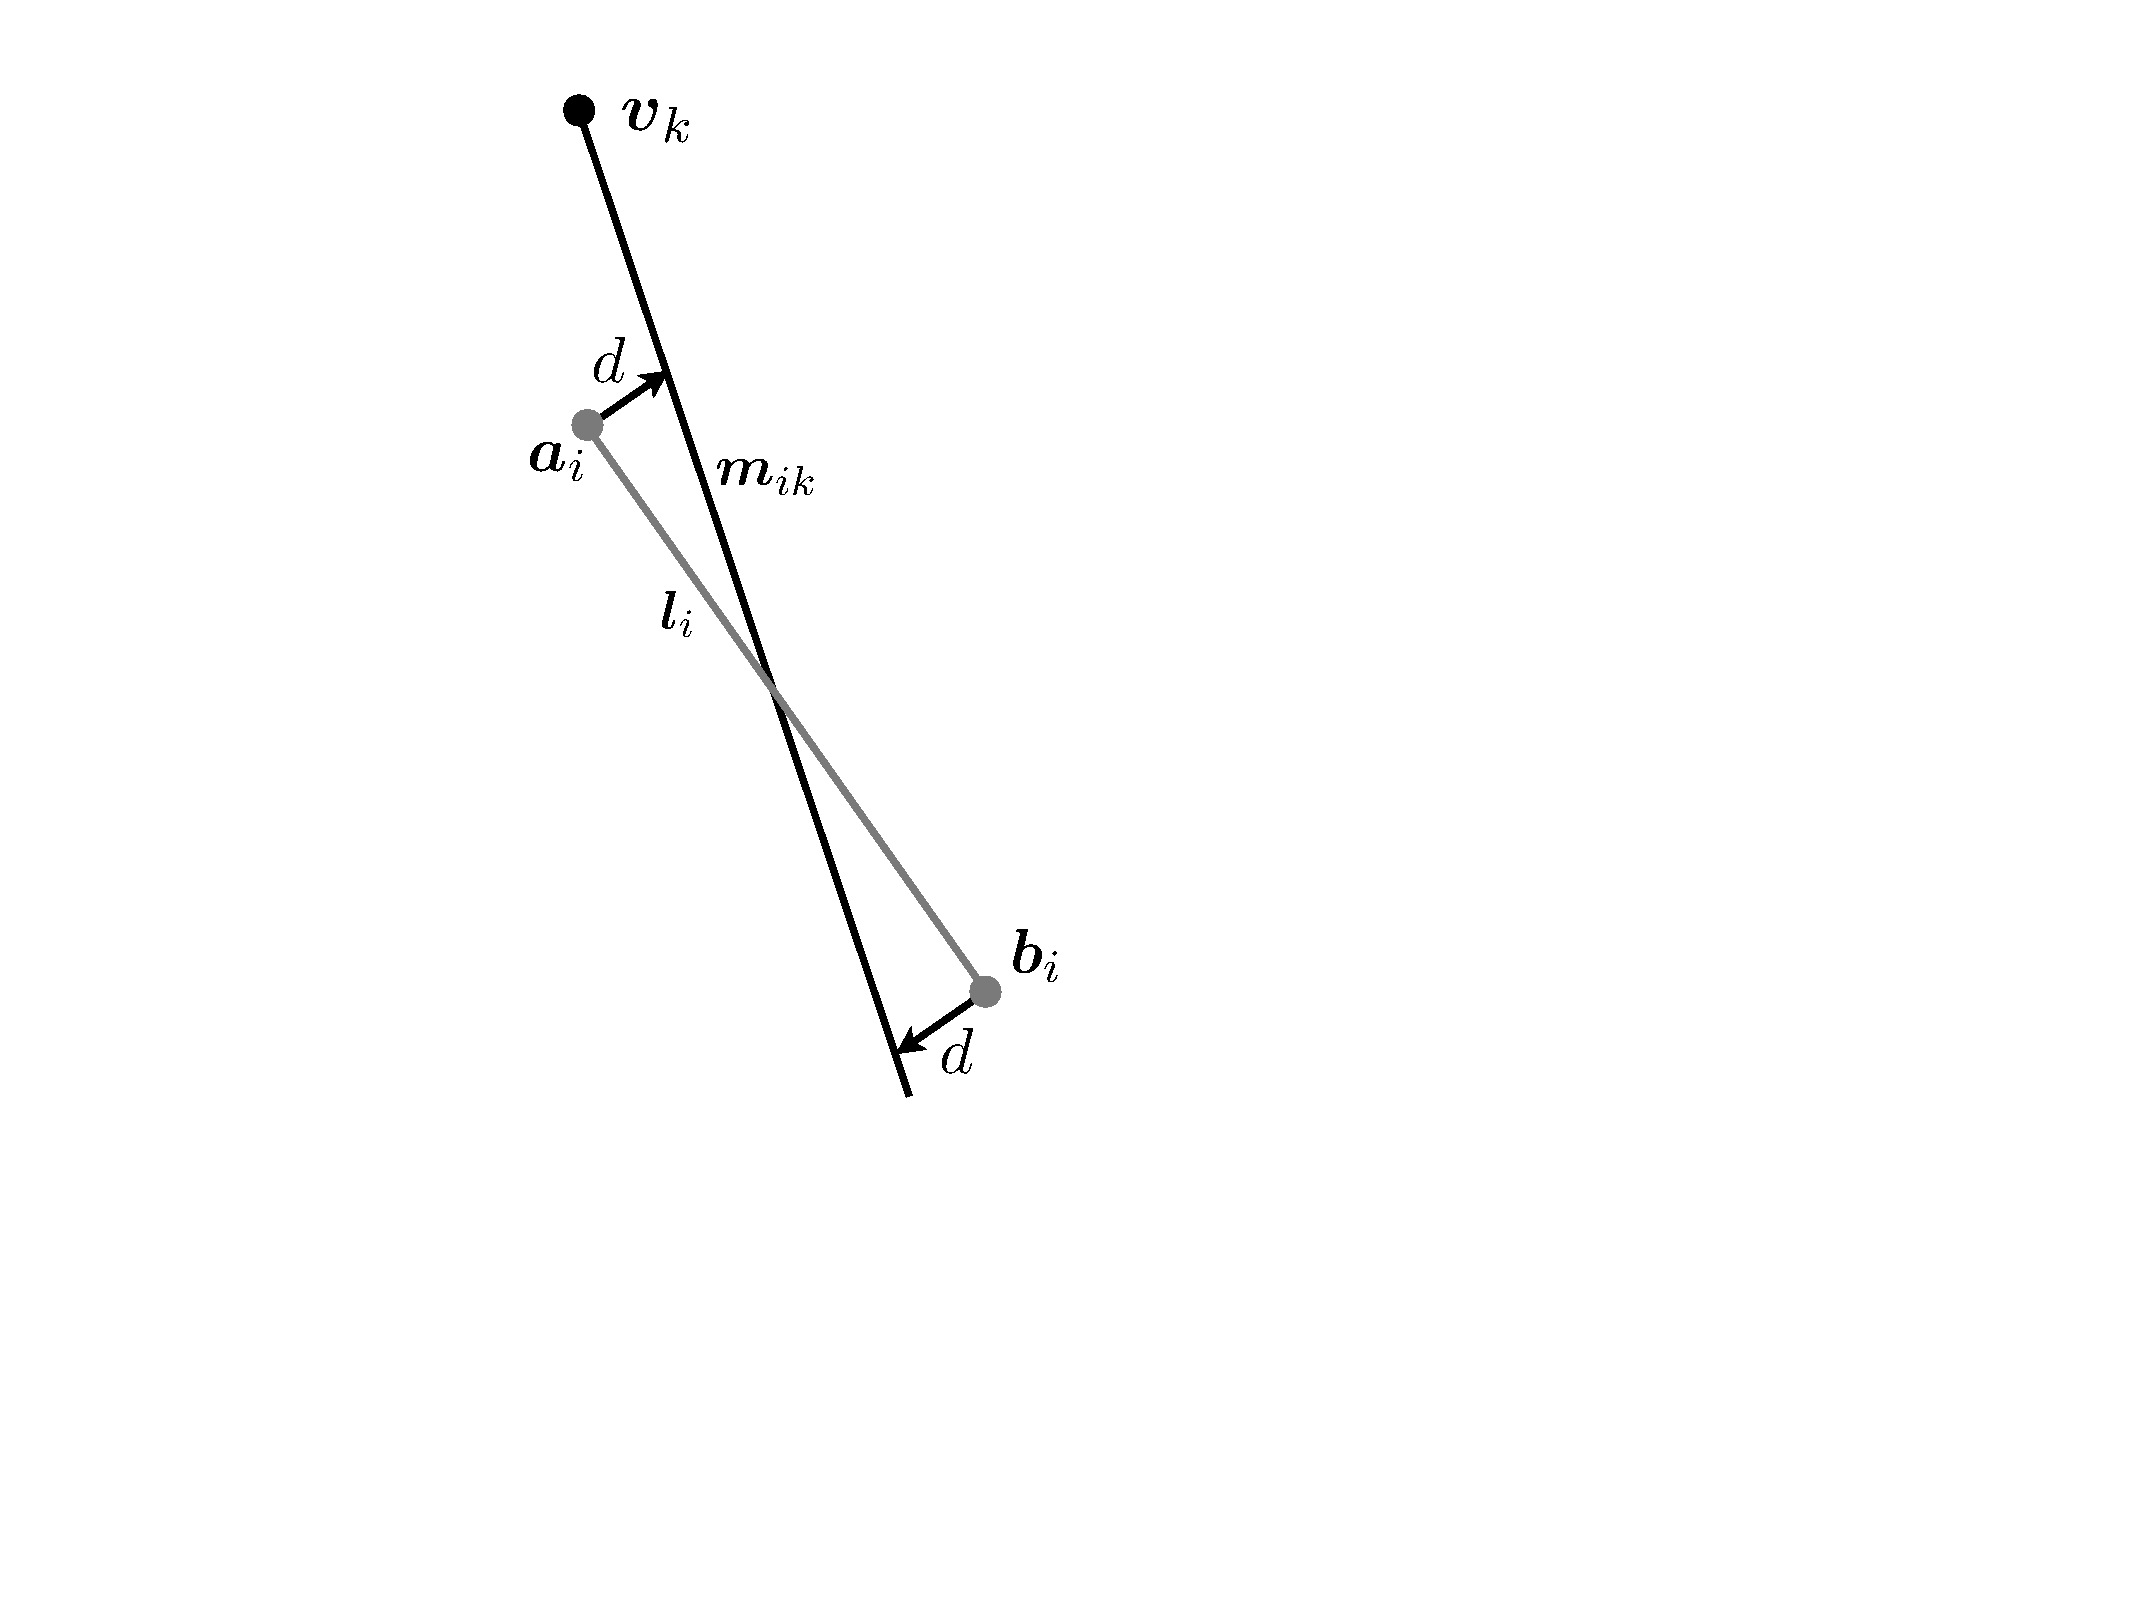
\includegraphics[width=0.4\textwidth]{reproj-dist}
  }  
  \caption{\changedsinceviva{Illustration of our error model and various geometric
    quantities involved in the derivations in the main text.}}
  \label{fig:line-model}
\end{figure}

We assume the graphical model shown in \figref{R-graphical}. The
generative process operates as follows. First we sample a scene
orientation $\SceneR$ and the rotation component of the camera pose,
$\CamR_j$ for each frame. (Camera translation plays no part when
reasoning about vanishing points.) Next we sample a discrete variable
$\Indicator_i$ from a categorical distribution with mixing parameters
$\Mixing$. The variable $\Indicator_i$ is a binary vector of length 4
indicating which vanishing point each line segment is associated
with. Exactly one element is set to 1, the other three are 0. The
first three elements correspond to the three vanishing points, the
fourth to a spurious observation not associated
with any of the three Manhattan directions. We denote the (binary)
value of the $k$\th element $\Indicator_{ik}$, but we will also write
$\Indicator_i=k$ as shorthand for the event that $\Indicator_i$ is the
binary vector with the $k$\th element set to 1. For clarity we write
$\Indicator_i=\Spurious$ in place of $\Indicator_i=4$. If
$\Indicator_i=\Spurious$ then the line segment $\TrueSeg_i$ is
sampled uniformly from the image. Otherwise, $\TrueSeg_i$ is
associated with the vanishing point $\vpt_{\Indicator_i}$ and is
sampled as follows.

The vanishing point corresponding to $\Indicator_i$ is
\begin{equation}
  \vpt_{\Indicator_i} = \CamR_j \SceneR \ebasis_{\Indicator_i} ~.
\end{equation}
We sample a ray through $\vpt$, then sample a line segment $\TrueSeg =
(\TrueStartPt,\TrueEndPt)$ along the ray. We add isotropic Gaussian
noise to arrive at the measured line segment
$\LineSeg=(\StartPt,\EndPt)$:
\begin{eqnarray}
  \StartPt &\sim& \NormalDistr(\TrueStartPt, \Sigma) \\
  \EndPt &\sim& \NormalDistr(\TrueEndPt, \Sigma) ~.
\end{eqnarray}
This process is illustrated by the graphical model in \figref{R-graphical}.

The likelihood for line segments is
\begin{equation}
  P(\LineSeg_i ~|~ \Indicator_i,\SceneR) =
  \NormalDistr(\dist(\LineSeg_i,\vpt_{\Indicator_i}); 0, \sigma)
\end{equation}
where $\dist(\LineSeg,\vpt)$ is the reprojection error illustrated in
\figref{line-model}. $\dist$ is computed as follows. First,
draw a line between the vanishing point $\vpt$ and the mid--point of
the line segment $\LineSeg$,
\begin{equation}
  \ReprojLine_{ik} =
  \vpt_k \cross \frac{\StartPt_i+\EndPt_i}{2}
\end{equation}
Now, $\dist$ is the distance between the line $\ReprojLine$ and either
of the two end points of $\LineSeg$ (the two quantities are equal, as
evident by inspecting \figref{line-model}). So
\begin{eqnarray}
  \dist(\LineSeg_i,\vpt_k) &=& 
  \frac
      {\StartPt_i \cdot \ReprojLine_{ik}}
      {(\StartPt_{i}\cdot\ez) \eta_{ik}}\\
      \eta_{ik} &=&
      \sqrt{(\ReprojLine_{ik} \cdot \ex)^2 +
        (\ReprojLine_{ik} \cdot \ey)^2}
      ~.
\end{eqnarray}

\section{Estimating the Manhattan Coordinate Frame}

We now turn to the inference algorithm that we use to find the
maximum--likelihood estimate of $\SceneR$ under the probabilistic
assumptions described in the previous section. We begin by running the
Canny edge detector \cite{Canny1986}, followed by an edge linking
algorithm \cite{Zhang02} to identify a set of straight line segments
$\LineSeg_j = \{\Pixel : \LineSeg_j\cdot\Pixel = 0\}$.

Under the model presented in the previous section, the
likelihood of $\SceneR$ is
\begin{equation}
  P(\LineSegs ~|~ \SceneR,\{\CamR_i\}) =
  \int P(\LineSegs,\Indicators ~|~ \SceneR,\{\CamR_i\})
  ~\intd\Indicators ~.
\end{equation}
For brevity we will omit the camera poses $\{\CamR_i\}$ in the
remainder of this section; it may be assumed that all probabilities
to follow are conditioned on $\{\CamR_i\}$.

The indicators $\Indicators$ are latent variables over which we need
to marginalise in order to perform inference on $\SceneR$. Integrating
explicitly is intractable so we turn to the
expectation--maximisation (EM) algorithm, which alternately refines
estimates of the posterior on $\Indicators$ (the ``E--step'') and
$\SceneR$ (the ``M--step'').

Due to the iterative nature of the EM algorithm we adopt superscript
notation for the scene rotation and indicators to make clear the
dependence between successive time steps. $\SceneR^t$ is the estimate
of the scene rotation at time $t$ and $\PosteriorEst^t$ is the
estimate for the posterior on $\Indicators$ at time $t$. Note that the
former is an estimate of a variable but the latter is an estimate of a
distribution. For notational convenience we will treat $\PosteriorEst$
as a continuous function, though of course in practice we really just
store sufficient statistics for $\PosteriorEst$. Also note that we
never actually store or estimate the values of the indicators
$\Indicators$, so we have no need for superscripts on this
variable. Although $\Indicators$ does appear in the derivations to
follow, in every equation we are either marginalising it out, or
defining a function over it.

\subsection{Complete Data Likelihood}

In sections to follow we will need to deal with the complete data
likelihood,
\begin{equation}
  P(\LineSegs,\Indicators ~|~ \SceneR) =
  \prod_i P(\LineSeg_i,\Indicator_i ~|~ \SceneR)
\end{equation}

The likelihood terms $P(\LineSeg_i,\Indicator_i ~|~ \SceneR)$ depend
on $\Indicator_i$ in a complicated way, since $\LineSeg_i$ is
drawn from a different distribution depending on $\Indicator_i$:
\begin{eqnarray}
  P(\LineSeg_i,\Indicator_i ~|~ \SceneR) &=&
  P(\Indicator_i ~|~ \SceneR)~
  P(\LineSeg_i, ~|~ \Indicator_i, \SceneR)\\
  &=&
  \begin{cases}
    \Mixing_1 
    \NormalDistr\bigr(\dist(\LineSeg_i, \CamR_i\SceneR\ex\bigl); 0,\sigma),
    & \mbox{if } \Indicator_i = 1 \\
    \Mixing_2
    \NormalDistr\bigr(\dist(\LineSeg_i, \CamR_i\SceneR\ey\bigl); 0,\sigma),
    & \mbox{if } \Indicator_i = 2 \\
    \Mixing_3
    \NormalDistr\bigr(\dist(\LineSeg_i, \CamR_i\SceneR\ez\bigl); 0,\sigma),
    & \mbox{if } \Indicator_i = 3 \\
    \Mixing_{\Spurious}
    \frac{1}{Z_\Spurious},
    & \mbox{if } \Indicator_i = \Spurious ~.
  \end{cases}
\end{eqnarray}
Due to our definition of $\Indicator_i$ as a binary vector we can
express this likelihood in the following analytic form,
\begin{equation}
  \label{eq:complete-likelihood}
  P(\LineSeg_i,\Indicator_i ~|~ \SceneR) =
  \prod_{k=1}^4 \Bigl( 
  P(\LineSeg_i ~|~ \Indicator_i=k,\SceneR)
  P(\Indicator_i=k ~|~ \SceneR)
  \Bigr)^{\Indicator_{ik}} ~.
\end{equation}

\subsection{The E--step}

During this phase we compute sufficient statistics for the posterior on
the indicators given a fixed estimate of $\SceneR$. This posterior
is
\begin{eqnarray}
  \PosteriorEst^t(\Indicators) &=&
  P(\Indicators ~|~ \LineSegs,\SceneR^t) \\
  \label{eq:posterior-est}
  &=&
  \frac{
    \prod_i P(\LineSeg_i,\Indicator_i ~|~\SceneR^t)
  }{
    \int \prod_i P(\LineSeg_i,\Indicator_i ~|~ \SceneR^t)
    ~\intd\Indicators
  }
\end{eqnarray}
Consider the term on the top line,
\begin{equation}
  P(\LineSeg_i,\Indicator_i ~|~\SceneR^t)
  =
  P(\LineSeg_i ~|~ \Indicator_i,\SceneR^t)
  P(\Indicator_i ~|~ \SceneR^t) ~.
\end{equation}
As a function of $\Indicator_i$ this is simply a categorical
distribution: $\Indicator_i$ can take on 3 possible values, and we can
compute each explicitly since $\SceneR^t$ and $\LineSeg_i$ are
fixed. Now since equation \eqnref{posterior-est} is a
normalised concatenation of categorical distributions, it is
itself a categorical distribution, meaning that the sufficient
statistics for $\PosteriorEst^t$ are the
expectations
\begin{eqnarray}
  \Expected_{\PosteriorEst^t}\bigl[ \Indicator_{ik} \bigr]
  &=& 
  \int \Indicator_{ik} \PosteriorEst^t(\Indicators) ~\intd\Indicators \\
  &=& 
  \sum_{\Indicator_{ik}\in\{0,1\}}
  \Indicator_{ik} P(\Indicator_{ik} ~|~ \LineSeg_i, \SceneR^t)\\
  &=&
  P(\Indicator_i=k ~|~ \LineSeg_i, \SceneR^t)\\
  &=&
  \label{eq:expected-zik}
  \frac
      {P( \LineSeg_i, \Indicator_i=k ~|~ \SceneR^t)}
      {\sum_{j=0}^4 P(\LineSeg_i, \Indicator_i=j ~|~ \SceneR^t)}
\end{eqnarray}
where in the third line we have expanded the sum over the two possible
values for $\Indicator_{ik}$ and cancelled the one in which
$\Indicator_{ik}$ is 0. Substituting the specific forms for the the
complete data likelihood \eqnref{complete-likelihood},
\begin{eqnarray}
  \Expected_{\PosteriorEst^t}\bigl[ \Indicator_{ik} \bigr] 
  &=&
  \frac{
    \prod_{k=1}^4\limits \Bigl( 
    P(\LineSeg_i ~|~ \Indicator_i=k,\SceneR^t)
    P(\Indicator_i=k ~|~ \SceneR^t)
    \Bigr)^{\Indicator_{ik}}
  }{
    \sum_{\Indicator_i=1}^4\limits
    \prod_{k=1}^4\limits \Bigl( 
    P(\LineSeg_i ~|~ \Indicator_i=k,\SceneR^t)
    P(\Indicator_i=k ~|~ \SceneR^t)
    \Bigr)^{\Indicator_{ik}}
  }\\
  \label{eq:big-expectation}
  &=&
  \frac{
    \Bigl(
    \Mixing_{\Spurious}
    P(\LineSeg_i ~|~ \Indicator_i=\Spurious,\SceneR^t)
    \Bigr)^{\Indicator_{ik}}
    \prod_{k=1}^3\limits \Bigl(
    \Mixing_k
    P(\LineSeg_i ~|~ \Indicator_i=k,\SceneR^t)
    \Bigr)^{\Indicator_{ik}}
  }{
    \sum_{\Indicator_i=1}^4\limits \Biggl[
      \Bigl(
      \Mixing_{\Spurious}
      P(\LineSeg_i ~|~ \Indicator_i=\Spurious,\SceneR^t)
      \Bigr)^{\Indicator_{ik}}
      \prod_{k=1}^3\limits \Bigl( 
      \Mixing_k
      P(\LineSeg_i ~|~ \Indicator_i=k,\SceneR^t)
      \Bigr)^{\Indicator_{ik}}
      \Biggr]
  }~.
\end{eqnarray}
We now define
\begin{eqnarray}
  \SpurJoint_i &=& 
  \Mixing_{\Spurious}
  P(\LineSeg_i ~|~ \Indicator_i=\Spurious,\SceneR^t) \\
  \SpurIndicator_i &=&
  \begin{cases}
    1, & \mbox{if } \Indicator_i = \Spurious \\
    0, & \mbox{otherwise}
  \end{cases}
\end{eqnarray}
and substituting into \eqnref{big-expectation} we have
\begin{eqnarray}
  \Expected_{\PosteriorEst^t}\bigl[ \Indicator_{ik} \bigr]
  &=&
  \frac{
    \SpurJoint_i^{\SpurIndicator_i}
    \Bigl(
    \Mixing_{\Indicator_i}
    \NormalDistr(\dist(\LineSeg,\CamR_i\SceneR^t\ebasis_k); 0, \sigma)
    \Bigr)^{1-\SpurIndicator_i}
  }{
    \sum_{\Indicator_i=1}^4\limits
    \SpurJoint_i^{\SpurIndicator_i}
    \Bigl(
    \Mixing_{\Indicator_i}
    \NormalDistr(\dist(\LineSeg,\CamR_i\SceneR^t\ebasis_{\Indicator_i}); 0, \sigma)
    \Bigr)^{1-\SpurIndicator_i}
  }\\
  &=&
  \frac{
    \SpurJoint_i^{\SpurIndicator_i}
    \Bigl(
    \Mixing_{\Indicator_i}
    \NormalDistr(\dist(\LineSeg,\CamR_i\SceneR^t\ebasis_k); 0, \sigma)
    \Bigr)^{1-\SpurIndicator_i}
  }{
    \SpurJoint_i +
    \sum_{\Indicator_i=1}^3\limits
    \Bigl(
    \Mixing_{\Indicator_i}
    \NormalDistr(\dist(\LineSeg,\CamR_i\SceneR^t\ebasis_{\Indicator_i}); 0, \sigma)
    \Bigr)
  }~.
  \label{eq:final-estep}
\end{eqnarray}
The E--step therefore consists of computing the expectations for
each indicator according to \eqnref{final-estep}, which are sufficient
statistics for the posterior on $\Indicators$. The expression
above can be evaluated for each indicator in constant time, leading to
a complexity for the E--step linear in the number of observed line
segments.

\subsection{M--step}
\label{sect:mstep}

During this phase we compute $\SceneR^{t+1}$ as the maximiser of the
expectation of the complete data log--likelihood under the (fixed)
distribution $\PosteriorEst^t$. The logarithm of the complete data
log--likelihood \eqnref{complete-likelihood} is
\begin{eqnarray}
  \log P(\LineSegs,\Indicators ~|~ \SceneR) 
  &=&
  \sum_i \sum_{k=1}^4 \Indicator_{ik} \Bigl(
  \log P(\LineSeg_i ~|~ \Indicator_i=k, \SceneR)
  + \log P(\Indicator_i=k ~|~ \SceneR)
  \Bigr)\\
  &=&
  \sum_i \sum_{k=1}^4 \Indicator_{ik} 
  \Bigl(
  \log \NormalDistr(\dist(\LineSeg_i, \CamR_i\SceneR\ebasis_k);0,\sigma)
  + \log \Mixing_k
  \Bigr)\\
  &=&
  \sum_i \sum_{k=1}^4 \Indicator_{ik} 
  \Bigl(
  \frac{-\dist(\LineSeg_i, \CamR_i\SceneR\ebasis_k)^2}{2\sigma^2}
  + \log \Mixing_k
  \Bigr) + c
\end{eqnarray}
where $c$ is a constant arising from the logarithm of the normal
distribution, which we now drop since it plays no part in the
maximisation to follow. The expectation of the above with respect to
the distribution $\PosteriorEst^t$ is
\begin{eqnarray}
  \Expected_{\PosteriorEst^t}\Bigl[
    \log P(\LineSegs,\Indicators ~|~ \SceneR) 
    \Bigr]
  &=&
  \sum_i \sum_{k=1}^4
  \Expected_{\PosteriorEst^t} \bigl[ \Indicator_{ik} \bigr]
  \Bigl(
  \frac{-\dist(\LineSeg_i, \CamR_i\SceneR\ebasis_k)^2}{2\sigma^2}
  + \log \Mixing_k
  \Bigr)\\
  &=&
  \label{eq:expected-lik}
  \sum_i \sum_{k=1}^4
  \Resp_{ik}^t
  \Bigl(
  \frac{-\dist(\LineSeg_i, \CamR_i\SceneR\ebasis_k)^2}{2\sigma^2}
  + \log \Mixing_k
  \Bigr)
\end{eqnarray}
where in the last line we have defined and substituted
\begin{equation}
  \Resp_{ik}^t = 
  \Expected_{\PosteriorEst^t} \bigl[ \Indicator_{ik} \bigr] ~.
\end{equation}

The maximisation we wish to perform is
\begin{equation}
  \label{eq:R-argmax}
  \SceneR^{t+1} = \argmax_{\SceneR}\limits
  \Expected_{\PosteriorEst^t}\Bigl[
    \log P(\LineSegs,\Indicators ~|~ \SceneR) 
    \Bigr] ~.
\end{equation}
It is worth examining the expression being maximised and noting which
variables it is and is not a function of. During each M--step, the
distribution $\PosteriorEst^t$, as represented by the sufficient
statistics computed in the E--step, is held fixed. The expectation is
over all possible values of the indicators $\Indicators$, each
weighted according to $\PosteriorEst^t$, which was computed from the
previous estimate $\SceneR^t$ but does not depend on the quantity
$\SceneR$ being maximised in this step. Hence the expression being
maximised in \eqnref{R-argmax} is a function of $\SceneR$ alone. Substituting
\eqnref{expected-lik},
\begin{eqnarray}
  \SceneR^{t+1} &=& \argmax_{\SceneR}\limits \ErrorFunc(\SceneR) \\
  \ErrorFunc(\SceneR) 
  &=&
  \label{eq:R-error}
  \sum_i \sum_{k=1}^4
  \Resp_{ik}^t
  \Bigl(
  \frac{-\dist(\LineSeg_i, \CamR_i\SceneR\ebasis_k)^2}{2\sigma^2}
  + \log \Mixing_k
  \Bigr)~.
\end{eqnarray}
Importantly, note that $\Resp_{ik}^t$ is a constant with respect to
$\SceneR$ in the above. We perform the maximisation
\eqnref{R-argmax} by gradient descent. Differentiating
\eqnref{R-error} with respect to $\SceneR$,
\begin{eqnarray}
  \Deriv{\ErrorFunc}{\SceneR}
  &=&
  \sum_i \sum_{k=1}^4
  \Resp_{ik}^t
  \Bigl(
  \frac{-\dist_{ik}}{\sigma^2}
  \Deriv{\dist_{ik}}{\SceneR} 
  \Bigr)\\
  \Deriv{\dist_{ik}}{\SceneR} &=&
  \frac{1}{\StartPt_i \cdot \ez} 
  \Biggl(
  % THIS NEGATION is swapped from some of the equations in my
  % notebook because the cross product matrix term at the end is negative
  \frac
      {(\ReprojLine_{ik})_1\ex + (\ReprojLine_{ik})_2\ey}
      {{\eta_{ik}}^3}
      (\ReprojLine_{ik} \cdot \StartPt_i)
      -
      \frac{\StartPt_i}{\eta_{ik}}
      \Biggr)
      \Bigl[ \frac{\StartPt_i+\EndPt_i}{2} \Bigr]_{\cross}
      \Deriv{\vpt_k}{\SceneR}
\end{eqnarray} 
where
\begin{eqnarray}
  \dist_{ik} &=& \dist(\LineSeg_i, \CamR_i\SceneR\ebasis_k)\\
  \eta_{ik} &=&
  \sqrt{(\ReprojLine_{ik} \cdot \ex)^2 +
    (\ReprojLine_{ik} \cdot \ey)^2}
\end{eqnarray}
and
\begin{equation}
  \bigl[ \vect{x} \bigr]_{\!\cross} = 
  \begin{bmatrix}
    0 & -x_3 & x_2 \\
    x_3 & 0 & -x_1 \\
    -x_2 & x_1 & 0
  \end{bmatrix}
\end{equation}
is the matrix form for the cross product.

For the purpose of optimisation we write $\SceneR$ as the product of a
fixed part $R_0$ and a variable part $R_{\delta}$, the latter of which
is represented in the Lie algebra for the special orthogonal group
$SO(3)$, so
\begin{eqnarray}
  \SceneR &=& R_0 R_{\delta} \\
  R_{\delta} &=& \exp\Bigl(\sum \LieM_i \Gen_i\Bigr)
\end{eqnarray}
where the $\Gen_i$ are the generator matrices for $SO(3)$ and the
$\LieM_i$ provide a minimal representation for the 3D rotation matrix
group. The advantage of using this representation is that after each
gradient step we are guaranteed that $\SceneR$ remains a pure
rotation, unlike under other representations such as optimising the
elements of the $3 \times 3$ rotation matrix directly. Differentiating
$\vpt$ with respect to $\LieMs$ yields
\begin{equation}
  \Deriv{\vpt_k}{\LieMs} = \CamR_i \Deriv{\SceneR}{\LieMs} \ebasis_k ~.
\end{equation}
The division of $\SceneR$ into fixed and variable parts allows us to
evaluate the gradient at $\LieMs=0$ without loss of generality. In
this case,
\begin{equation}
  \Deriv{\vpt_k}{\LieMs} \EvalAt{\LieMs=0} =
  \begin{bmatrix}
    \CamR_i R_0 \Gen_1 \ebasis_k &
    \CamR_i R_0 \Gen_2 \ebasis_k &
    \CamR_i R_0 \Gen_3 \ebasis_k
  \end{bmatrix}~.
\end{equation}

This completes the derivation of the gradient of the error function
$\ErrorFunc$ with respect to the parametrisation $\LieMs$. We proceed as
normal with gradient steps of the form
\begin{equation}
  \LieMs^{t+1} = \LieMs^t - \gamma \Deriv{\ErrorFunc}{\LieMs} ~.
\end{equation}

Due to the low dimensionality of the search space and relatively low
curvature of the error function we found that a simple instantiation
of the gradient descent algorithm converged quickly and robustly. Our
algorithm initialises the step size $\gamma$ to a fixed constant
$\gamma_0$ at the beginning of each M--step, then divides $\gamma$ by
2 each time that an update leads to an increase in the error
function. Convergence is detected when $\gamma<\epsilon_1$ and the
value of the error function decreases by less than $\epsilon_2$ in any
one update.

\subsection{Initialisation}

\changedsinceviva{
We initialise our EM algorithm using the clustering approach described
by Koseck\`{a} and Zhang \cite{Zhang02}. This process begins by
clustering observed line segments according to their orientation in
the image plane, the basis for this being that Manhattan environments
often contain Manhattan--oriented lines that are close to one another
(relative to the distance to the vanishing point), and hence appear
almost parallel. We run K--means clustering on all line segments in
each image separately (with $K=5$) then we estimate a least--squares
vanishing point for each cluster that has at least 5 associated line
segments. Finally we project vanishing points from all frames onto the
plane at infinity and pick three that are close to mutually orthogonal
(by enumerating all combinations). We initialise the EM algorithm with
an (orthonormalized) rotation matrix containing the chosen vanishing
points as columns.
}

\subsection{Summary}
To obtain $\SceneR$ we iterate between updating $\PosteriorEst$ (the
E--step) and optimising $\SceneR$ (the M--step). Each M step consists
of a gradient descent in the Lie group $SO(3)$. In practice we find
that our system converged in around 25 iterations of the EM algorithm,
and that approximately 10 steps were required for each gradient
descent.

\section{Results}

We evaluated our approach using a dataset of 18 video sequences of 8
unique places, which we collected in indoor environments such as homes
and office spaces. We ran \changedsinceviva{an} off--the--shelf bundle
adjuster on each sequence to yield calibrated views, then transformed
each sequence by a random 3D rotation to eliminate any bias in the
initial conditions for our optimisation that might have been
introduced by structure--from--motion. We manually provided the ground
truth scene orientation $\SceneR$ for each sequence. We sampled frames
at regular intervals of approximately one second, then divided all
sequences into successive 7--frame blocks. Each such block is a single
``evaluation instance'' in our dataset.

We compared four approaches including our own. First, the
surface--normal--based approach of \cite{Furukawa09} described at the
beginning of this chapter, which we refer to by symbol ``NRM''. For
each evaluation instance, this algorithm received as input all
reconstructed 3D points that were visible in any of the 7 views in
that instance. We were generous to this approach here since the
reconstruction of some of these points may have relied upon data from
other frames. Second, we tested a system identical
to ours but in which the reconstruction error was replaced by the
algebraic error --- we refer to this system as ``ALG'' below. Finally, we
evaluated our own system using both a single input view (``SIN''), and
all 7 views (``MUL''). The former approach is hence similar to that of
Schindler and Dellaert \cite{Schindler2004}.

The metric we used to compare the estimated and ground truth
rotations was
\begin{equation}
  \| R_1^T R_2 - I \|_{\mathcal{F}} ~.
  \label{eq:rotation-metric}
\end{equation}
where $\|\cdot\|_{\mathcal{F}}$ denotes the Frobenius norm. We chose
this metric because it was shown by Huynh \cite{Huynh2009} to be
iso--equivalent to many 3D rotation metrics in common usage within
the computer vision literature, including quaternion norms and inner
products, and metrics based on Euler angles and the Lie algebra
$so(3)$.

\tableref{rot-performance} summarises the performance of each
algorithm. Unsurprisingly, the surface normal approach fails under the
sparse structure--from--motion point clouds --- it was proposed in the
context of dense reconstructions. Strikingly, the multiple--view
algebraic minimiser performs consistently worse than single--image
estimation. \changedsinceviva{Our investigations suggest that this is because the
algebraic error is an even poorer approximation to the reprojection
error in the multiple view context than in the single--view context,
since among many frames there is a high likelihood of observing a
vanishing point close to infinity. As a vanishing point moves towards
infinity, the algebraic error diverges from the reprojection error,
and the error terms for vanishing points near infinity to dominate the
objective function. This leads to poorly reconstructed vanishing
points since the optimisation focuses almost exclusively on these
very large error terms, ignoring the majority of the image evidence.
}

We ran a separate experiment to explore the relationship between the
number of frames used for estimation and the quality of the estimated
rotation; these results are shown in \figref{error-vs-nframes}. As the
number of frames used for estimation increases, the quality of the
estimator described in this chapter improves as expected. However, it
is interesting to note that the algebraic minimiser actually degrades
for more than 5 input frames. This supports our hypothesis above that
the algebraic error is an even poorer choice in the multiple--view
context than for single images.

Our third experiment explored the convergence properties of the
gradient descent component of our optimisation. Starting from an
initial rotation a specified distance from the ground truth, we
plotted the progress of our algorithm after each gradient step
(\figref{rotation-convergence}). In this experiment the indicators
$\Indicators$ were assumed known. Progress was measured both in terms
of the log--likelihood, which the optimiser itself has access to
(lower figure), and distance to ground truth, which the optimiser
obviously does not have access to (upper figure). This experiment
shows two things. First, that the basin of attraction is very wide ---
convergence is robust for distances up to $1.0$, which is a large
distance in the metric \eqnref{rotation-metric}. Second, that the
log-likelihood accurately tracks the ground truth error in practice,
since the runs that did not converge to the ground truth also
terminated at much lower log--likelihoods.

Finally, examples of the output from the four systems described above
are shown in Figures \ref{fig:vpt-example1}, \ref{fig:vpt-example2},
and \ref{fig:vpt-example3}.


%\figref{bathroom-vpts} shows the vanishing points identified in one of
%our sequences. Since each frame is informed by the entire sequence we
%are able to identify a globally consistent coordinate frame where
%single--image vanishing point detection fails. \figref{vpt-comparison}
%shows a side--by--side comparison with the single--image vanishing
%point detector of \cite{Zhang02}. Recently proposed improvements to
%the single--image approach \cite{Tardif09} may improve slightly on
%these, but we found that in cases where the single--image approach
%fails there is often simply not enough information available in
%individual frames to identify the appropriate coordinate frame, so any
%single--image approach will necessarily fail.

\begin{table}[tb]
  \centering
  \begin{tabular}{@{}p{2cm}p{3cm}p{3cm}p{3cm}p{3cm}@{}}
    \toprule
    Sequence & Error for NRM & Error for ALG & Error for SIN & Error
    for MUL \\
    \midrule
    \tt{Kitchen}  & 0.53   & 0.59   & 0.037  & \textbf{0.019} \\
    \tt{Foyer 1}   & 0.72   & 0.77   & 0.054  & \textbf{0.039} \\
    \tt{Foyer 2}  & 0.81   & 0.75   & 0.070  & \textbf{0.021} \\
    \tt{Bursary}  & 0.50   & 0.53   & 0.067  & \textbf{0.030} \\
    \tt{Ground}   & 0.90   & 0.68   & \textbf{0.55}   & 0.66 \\
    \tt{Atrium}   & 0.84   & 1.00   & 0.31  & \textbf{0.16} \\
    \tt{MCR}      & 0.56   & 0.56   & 0.06  & \textbf{0.04} \\
    \tt{Corridor} & 0.58   & 0.78   & \textbf{0.20}  & 0.21 \\
    \bottomrule
  \end{tabular}
  \vspace{0.2cm}
  \caption{Distance between estimated and ground truth rotation for
    four algorithms. Each cell shows the average error over all frames
    within a given sequence. From left to right the algorithms are
    the point--cloud procedure of \cite{Furukawa09} (NRM),
    Expectation--Maximisation using the algebraic error (ALG),
    Expectation--Maximisation using the geometric error applied to
    single (SIN) and multiple (MUL) images. All algorithms other than
    SIN were given 7 input frames in this experiment.}
  \label{table:rot-performance}
\end{table}

\begin{figure}[p]
  \centering
  \subfloat[Estimation error versus number of input frames.]{
    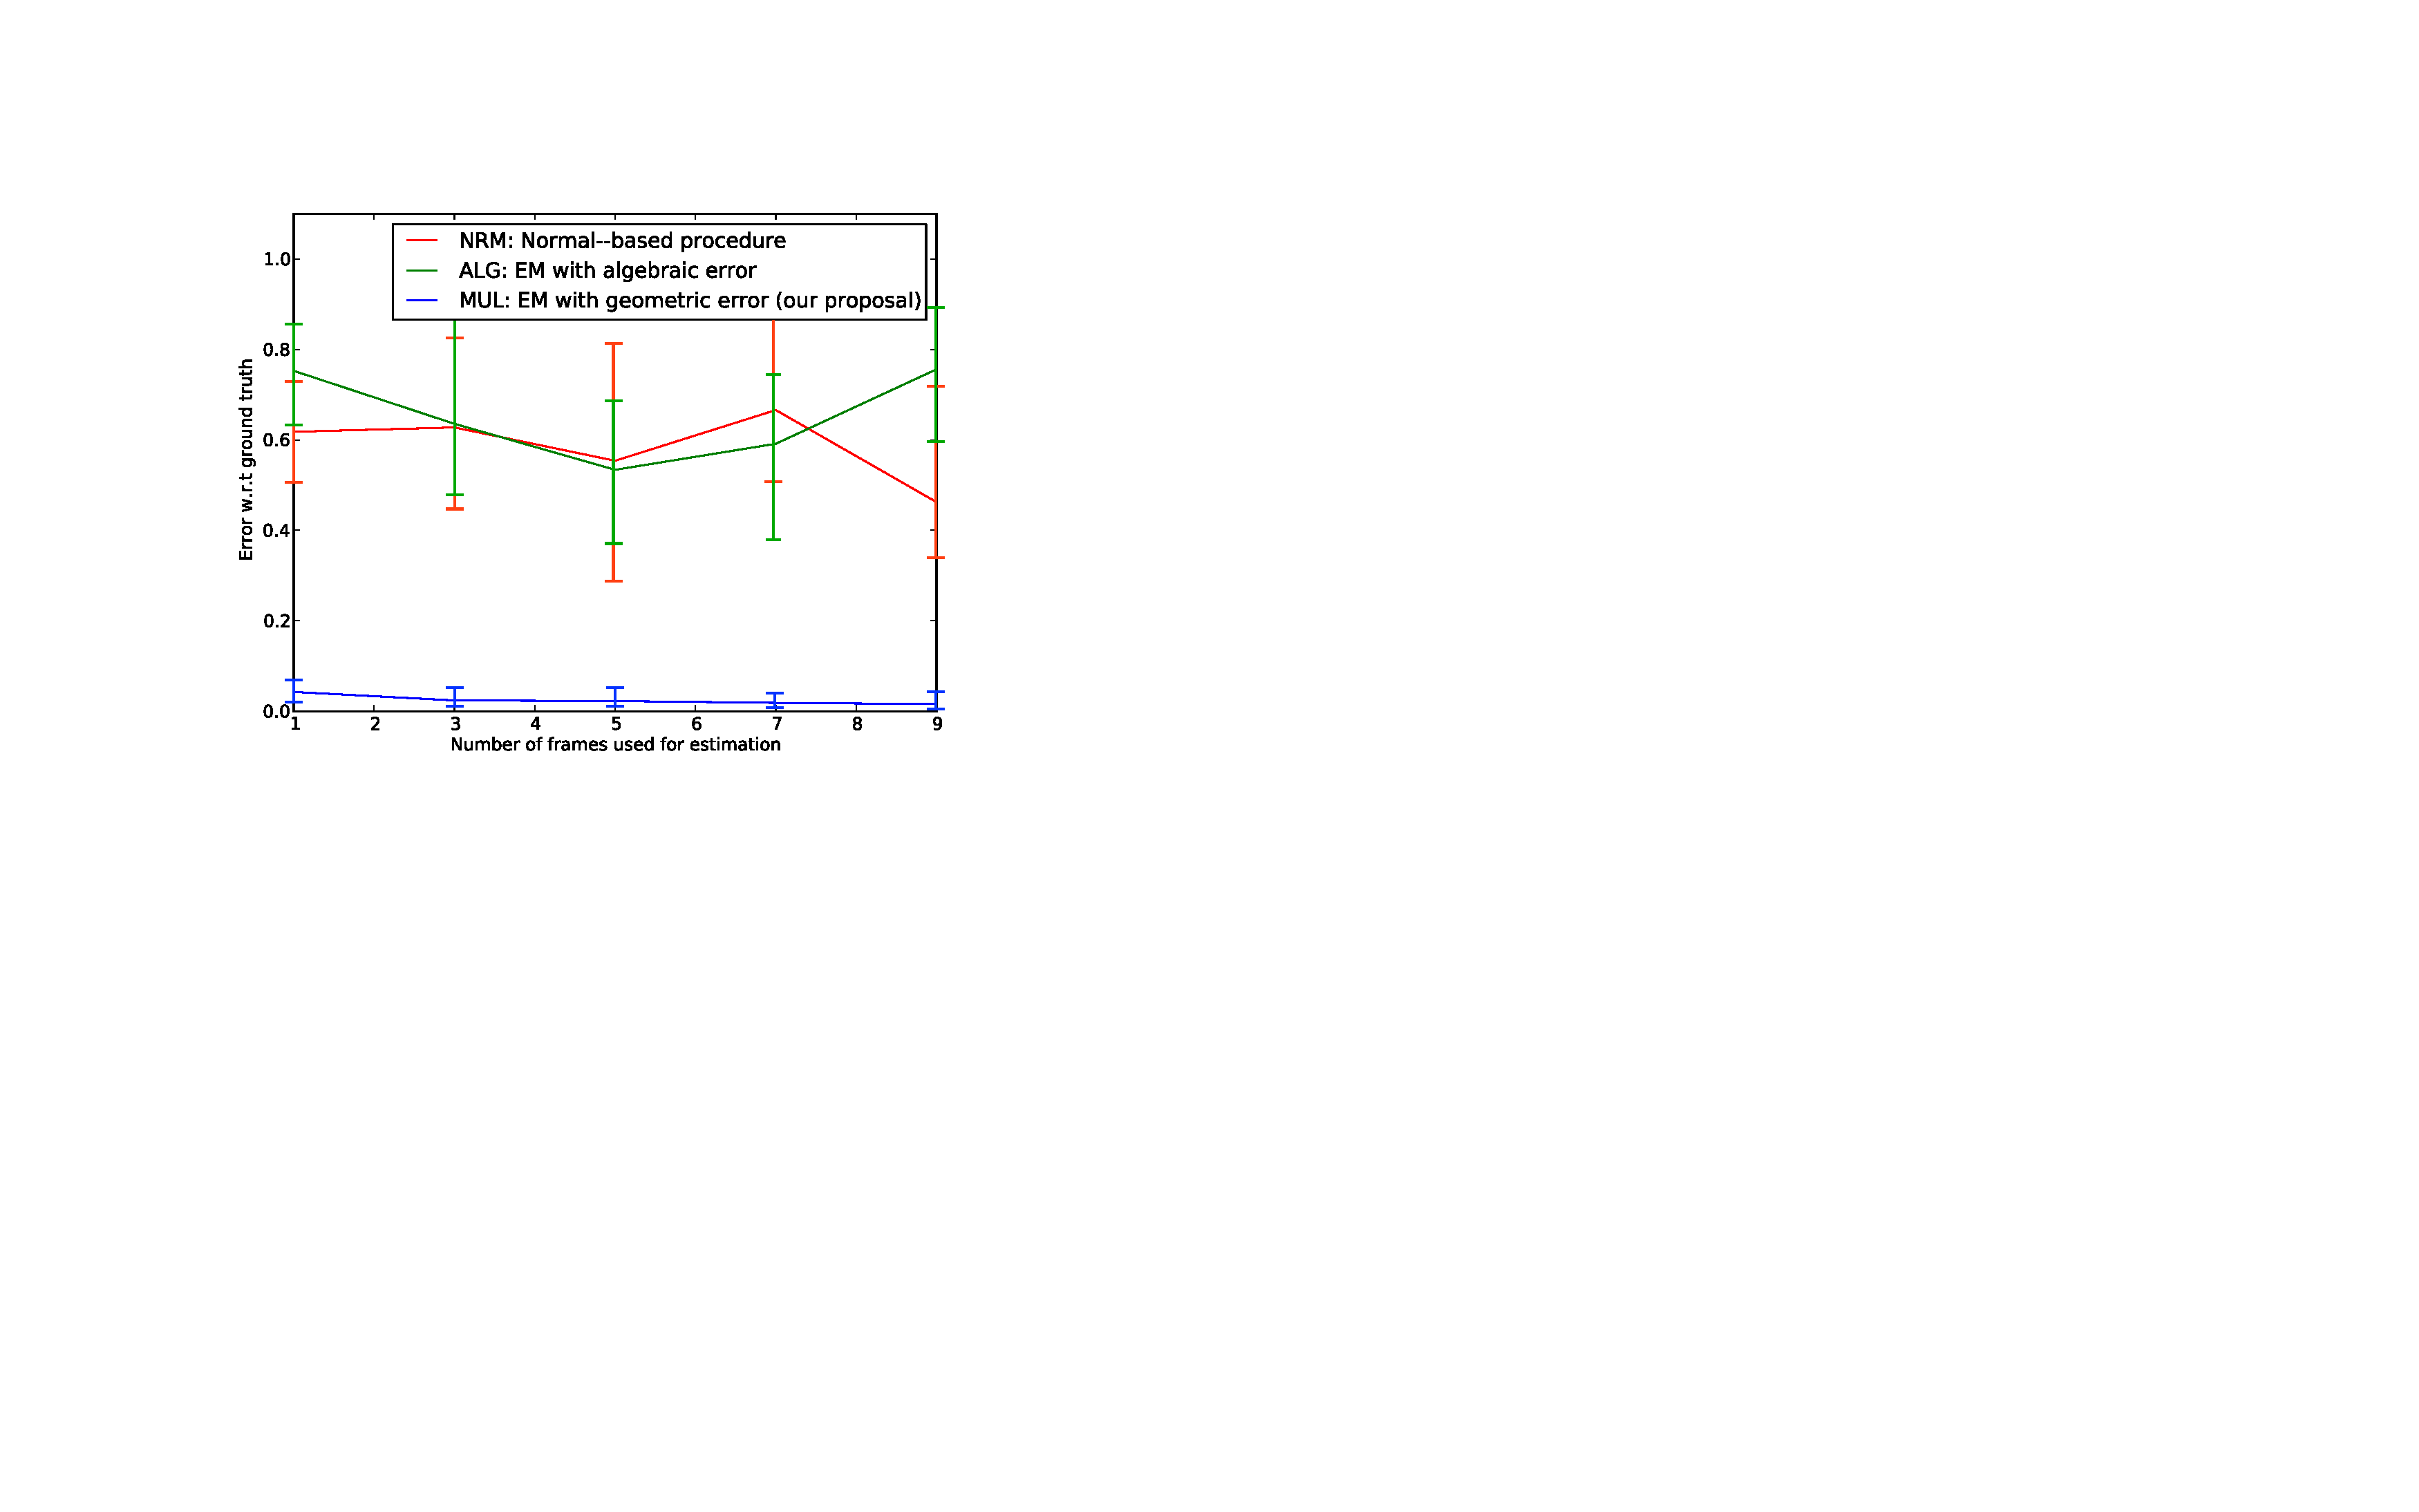
\includegraphics[width=0.65\textwidth]{plots/error_vs_nframes_with_errorbars}
  }
  \\
  \subfloat[A magnification of the third series above.]{
    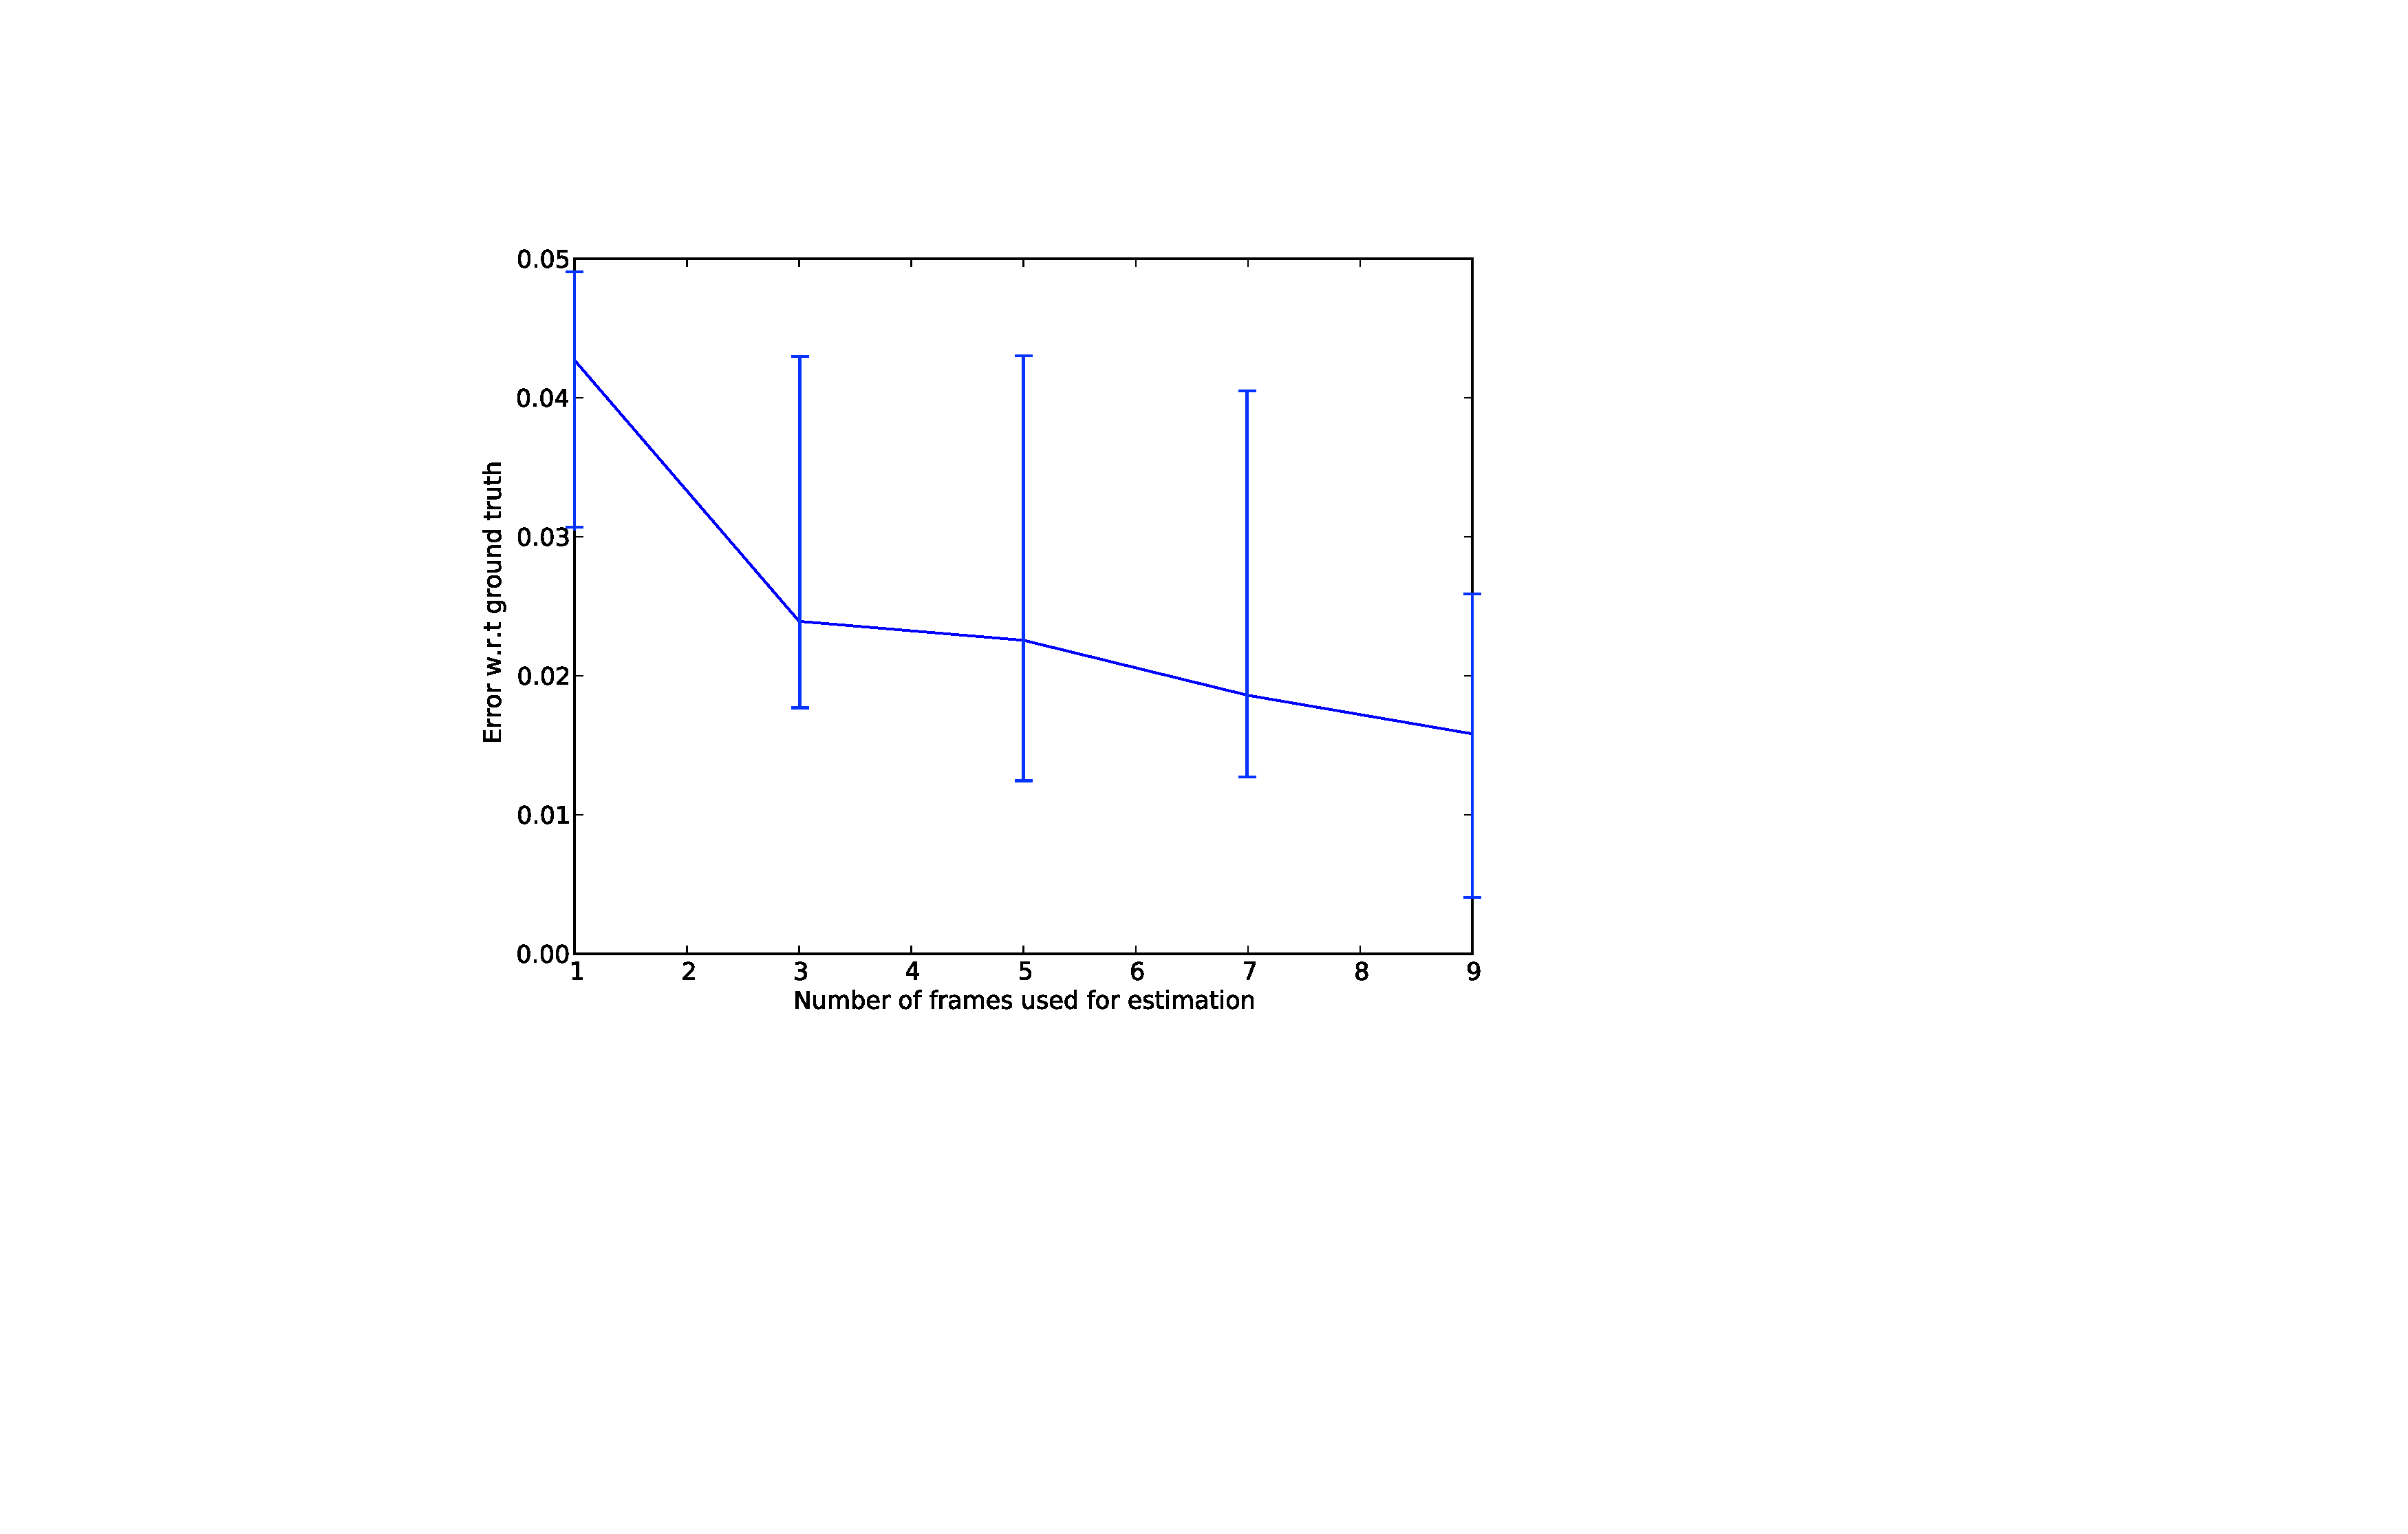
\includegraphics[width=0.65\textwidth]{plots/error_vs_nframes_oursonly_with_errorbars}
  }
  \caption{\changedsinceviva{Plots showing the performance of three algorithms as the
    number of input frames is increased. We compute each data point by
    executing the relevant algorithm on sets of $n$ consecutive frames
    drawn from our dataset, where $n$ is the value shown on the
    $x$--axis. The $y$--axis shows the average distance between the
    estimated and ground truth rotation, with error bars showing 90\%
    confidence intervals for the observed error distributions.}}
  \label{fig:error-vs-nframes}
\end{figure}


\begin{figure}[tb]
  \centering
  \subfloat[Convergence of error (with respect to ground truth)]{
    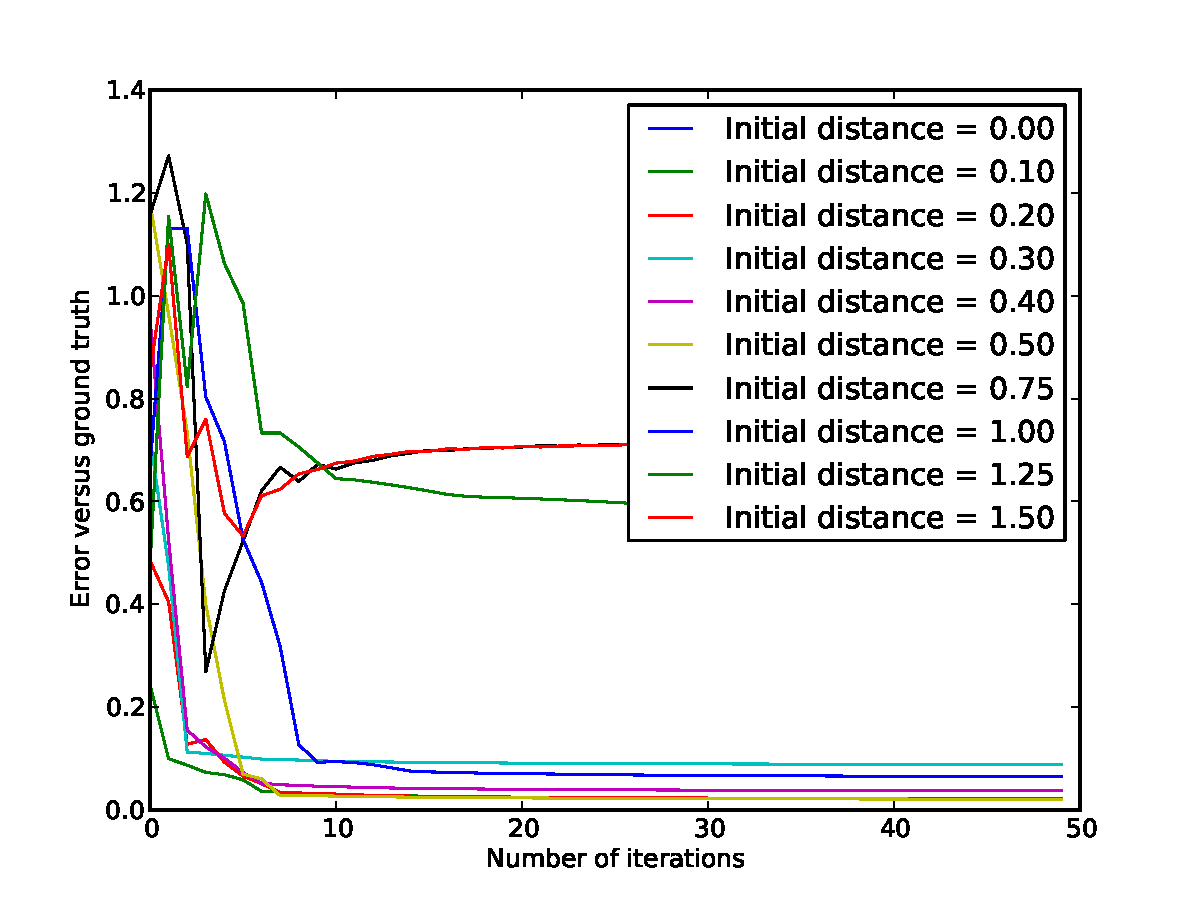
\includegraphics[width=0.65\textwidth]{plots/rotation_convergence_gterror}
  }
  \\
  \subfloat[Convergence of log--likelihood]{
    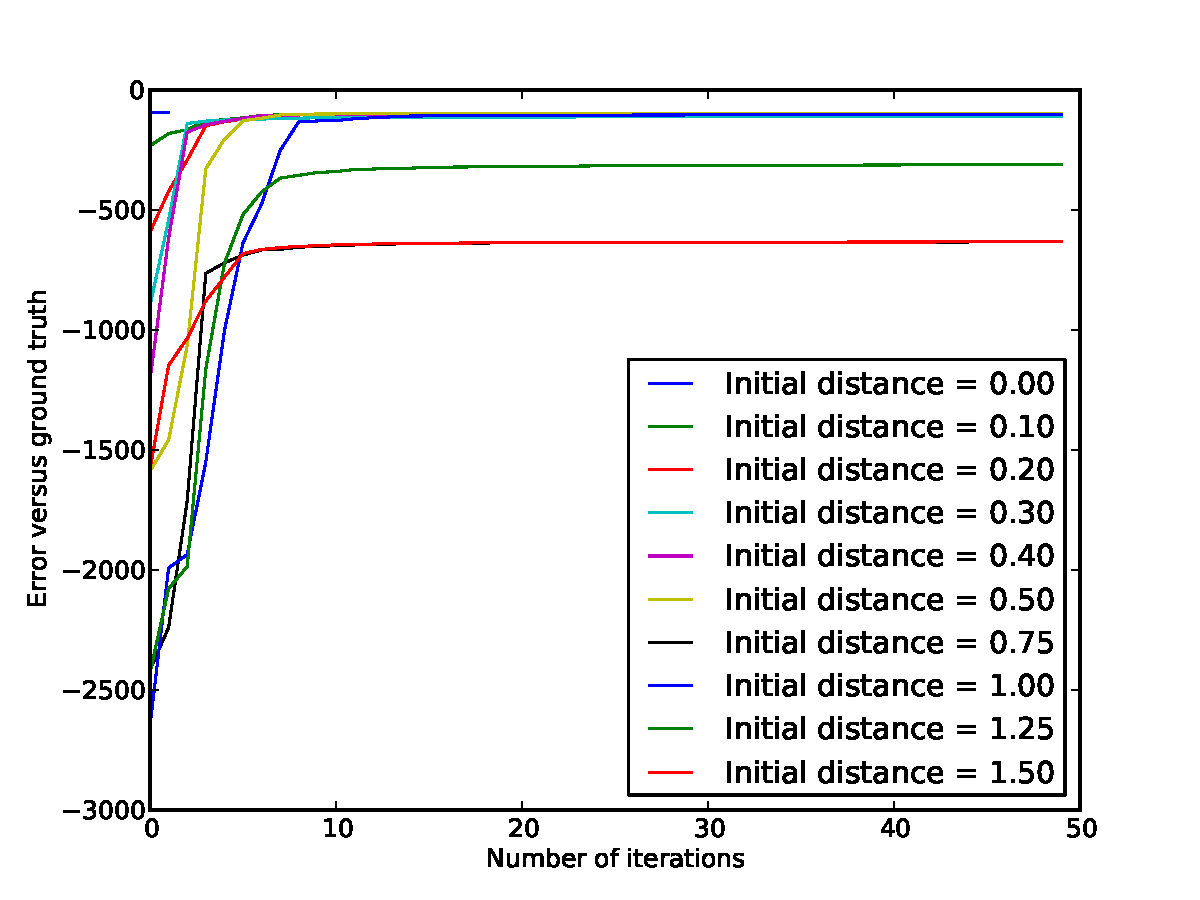
\includegraphics[width=0.65\textwidth]{plots/rotation_convergence_likelihood}
  }
  \caption{Illustration of the convergence properties of our gradient
    descent algorithm. We measure the distance from the estimated
    rotation to the ground truth after each gradient step. Each series
    above shows this evolution when our algorithm is initialised a
    particular distance from the ground truth. We see that for
    distances less than 1 convergence is robust. This corresponds to a
    large offset under the metric \eqnref{rotation-metric}, indicating
    that the optima has a wide basin of attraction. Note that for this
    experiment the labels $\Indicators$ are assumed known.}
  \label{fig:rotation-convergence}
\end{figure}

\begin{figure}[p]
  \centering
  \subfloat[Algebraic Estimate]{
    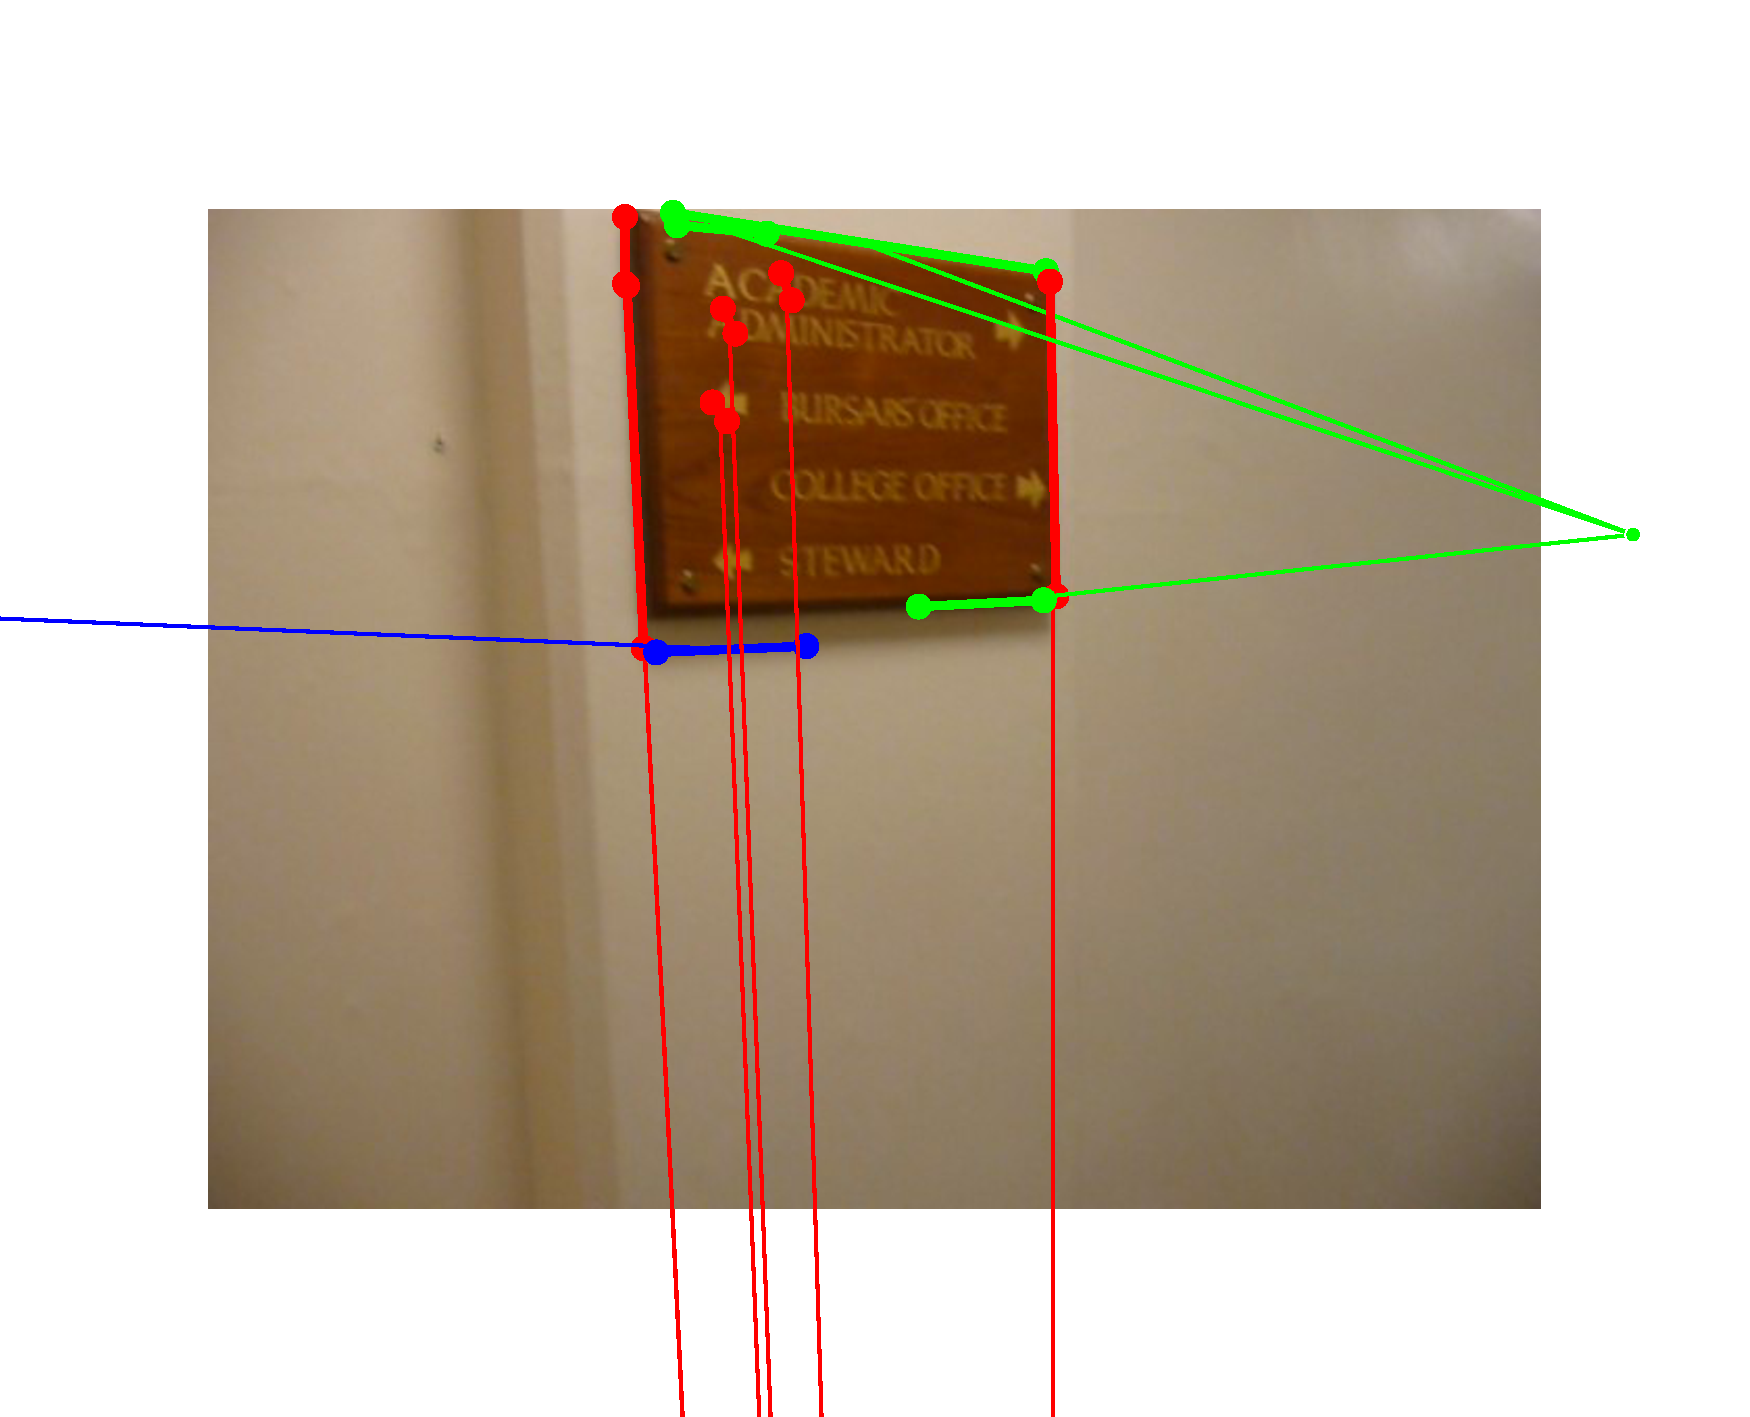
\includegraphics[width=0.46\textwidth]{new_vpt_comparison/exeter_bursary_frame23_vpts_algebraic}
  }\quad
  \subfloat[Normal--based Estimate]{
    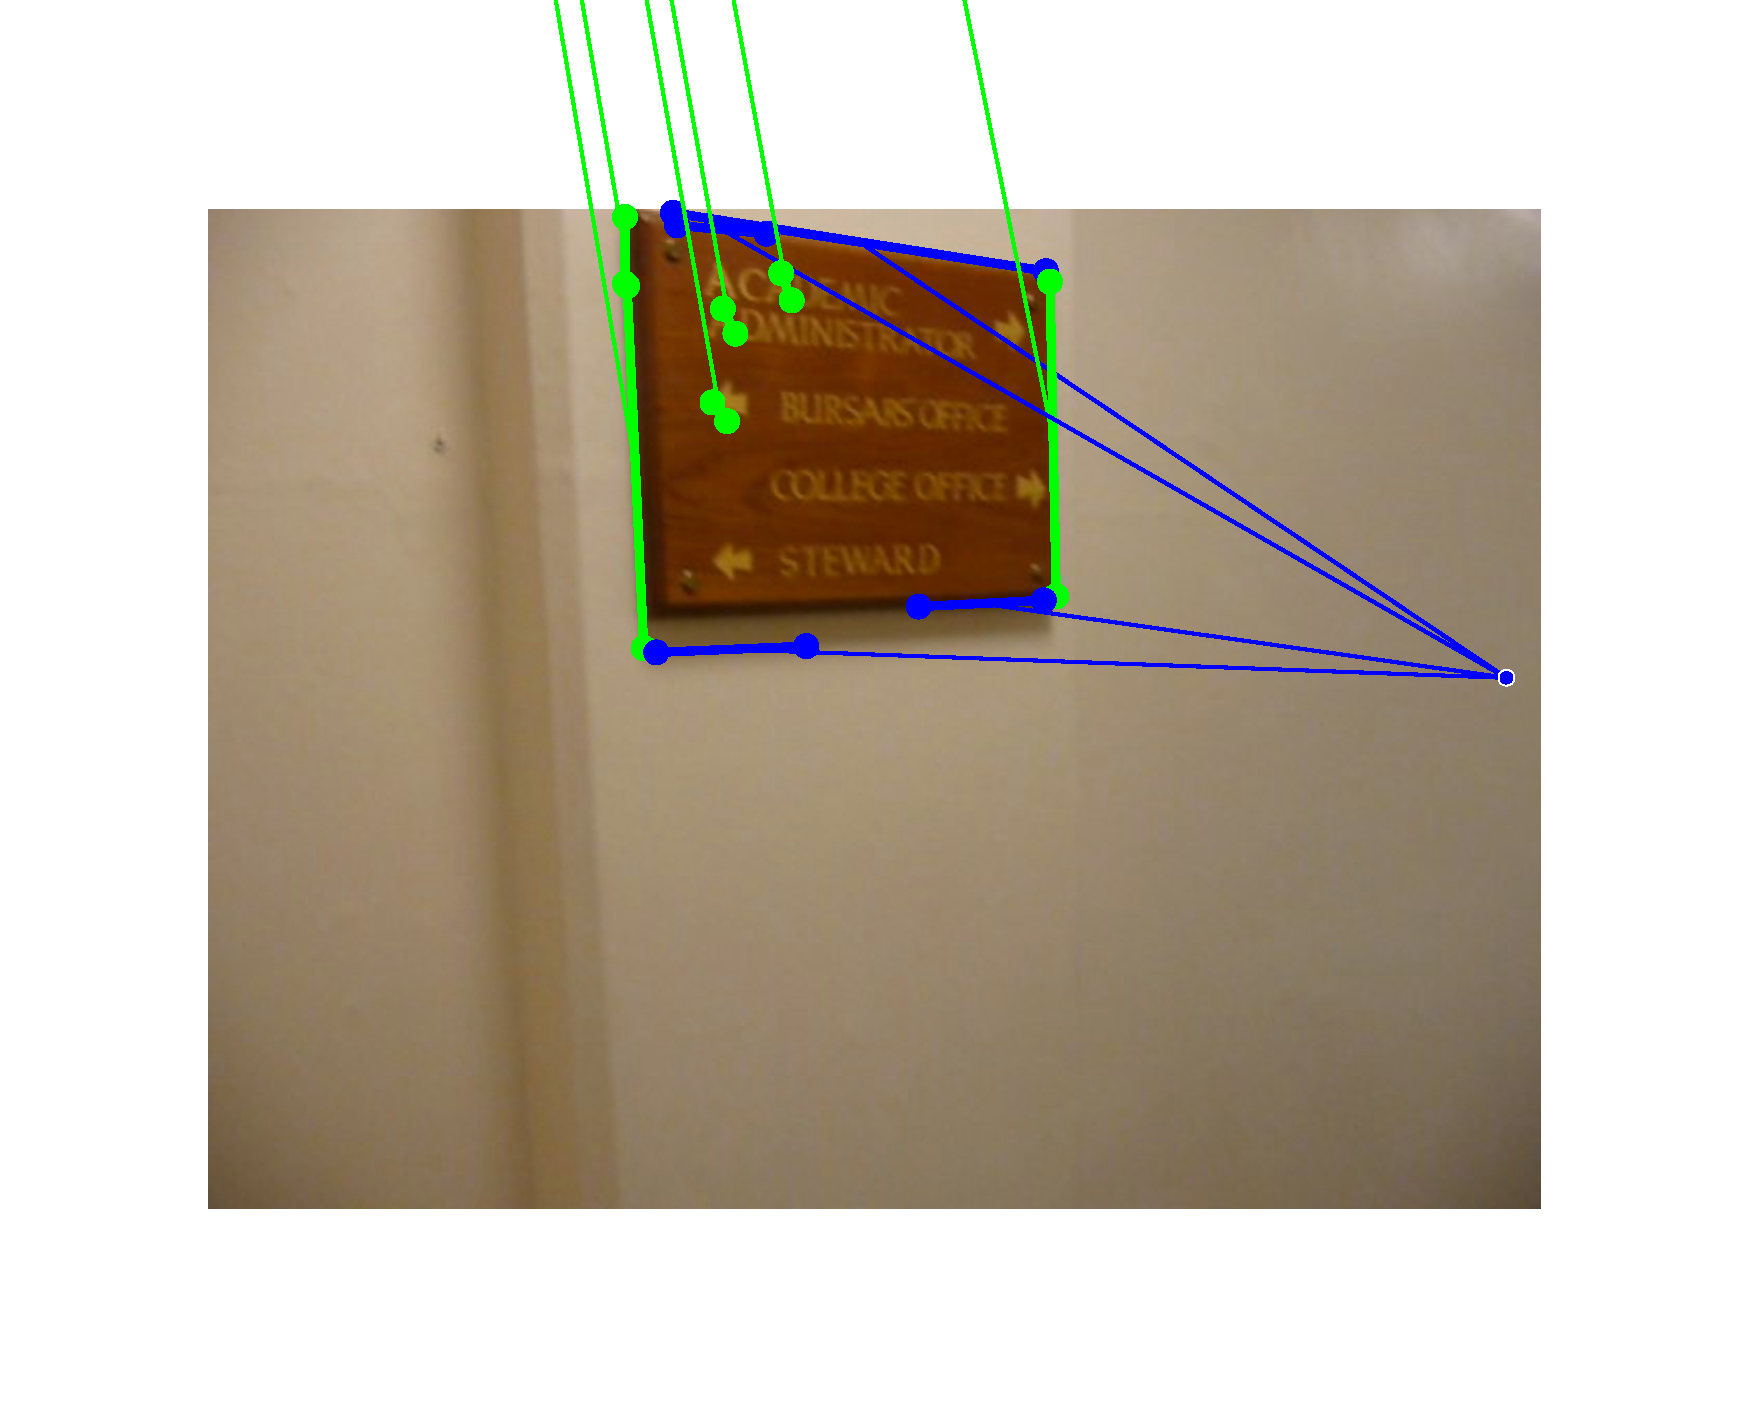
\includegraphics[width=0.46\textwidth]{new_vpt_comparison/exeter_bursary_frame23_vpts_normals}
  }\\
  \subfloat[Single Image Estimate]{
    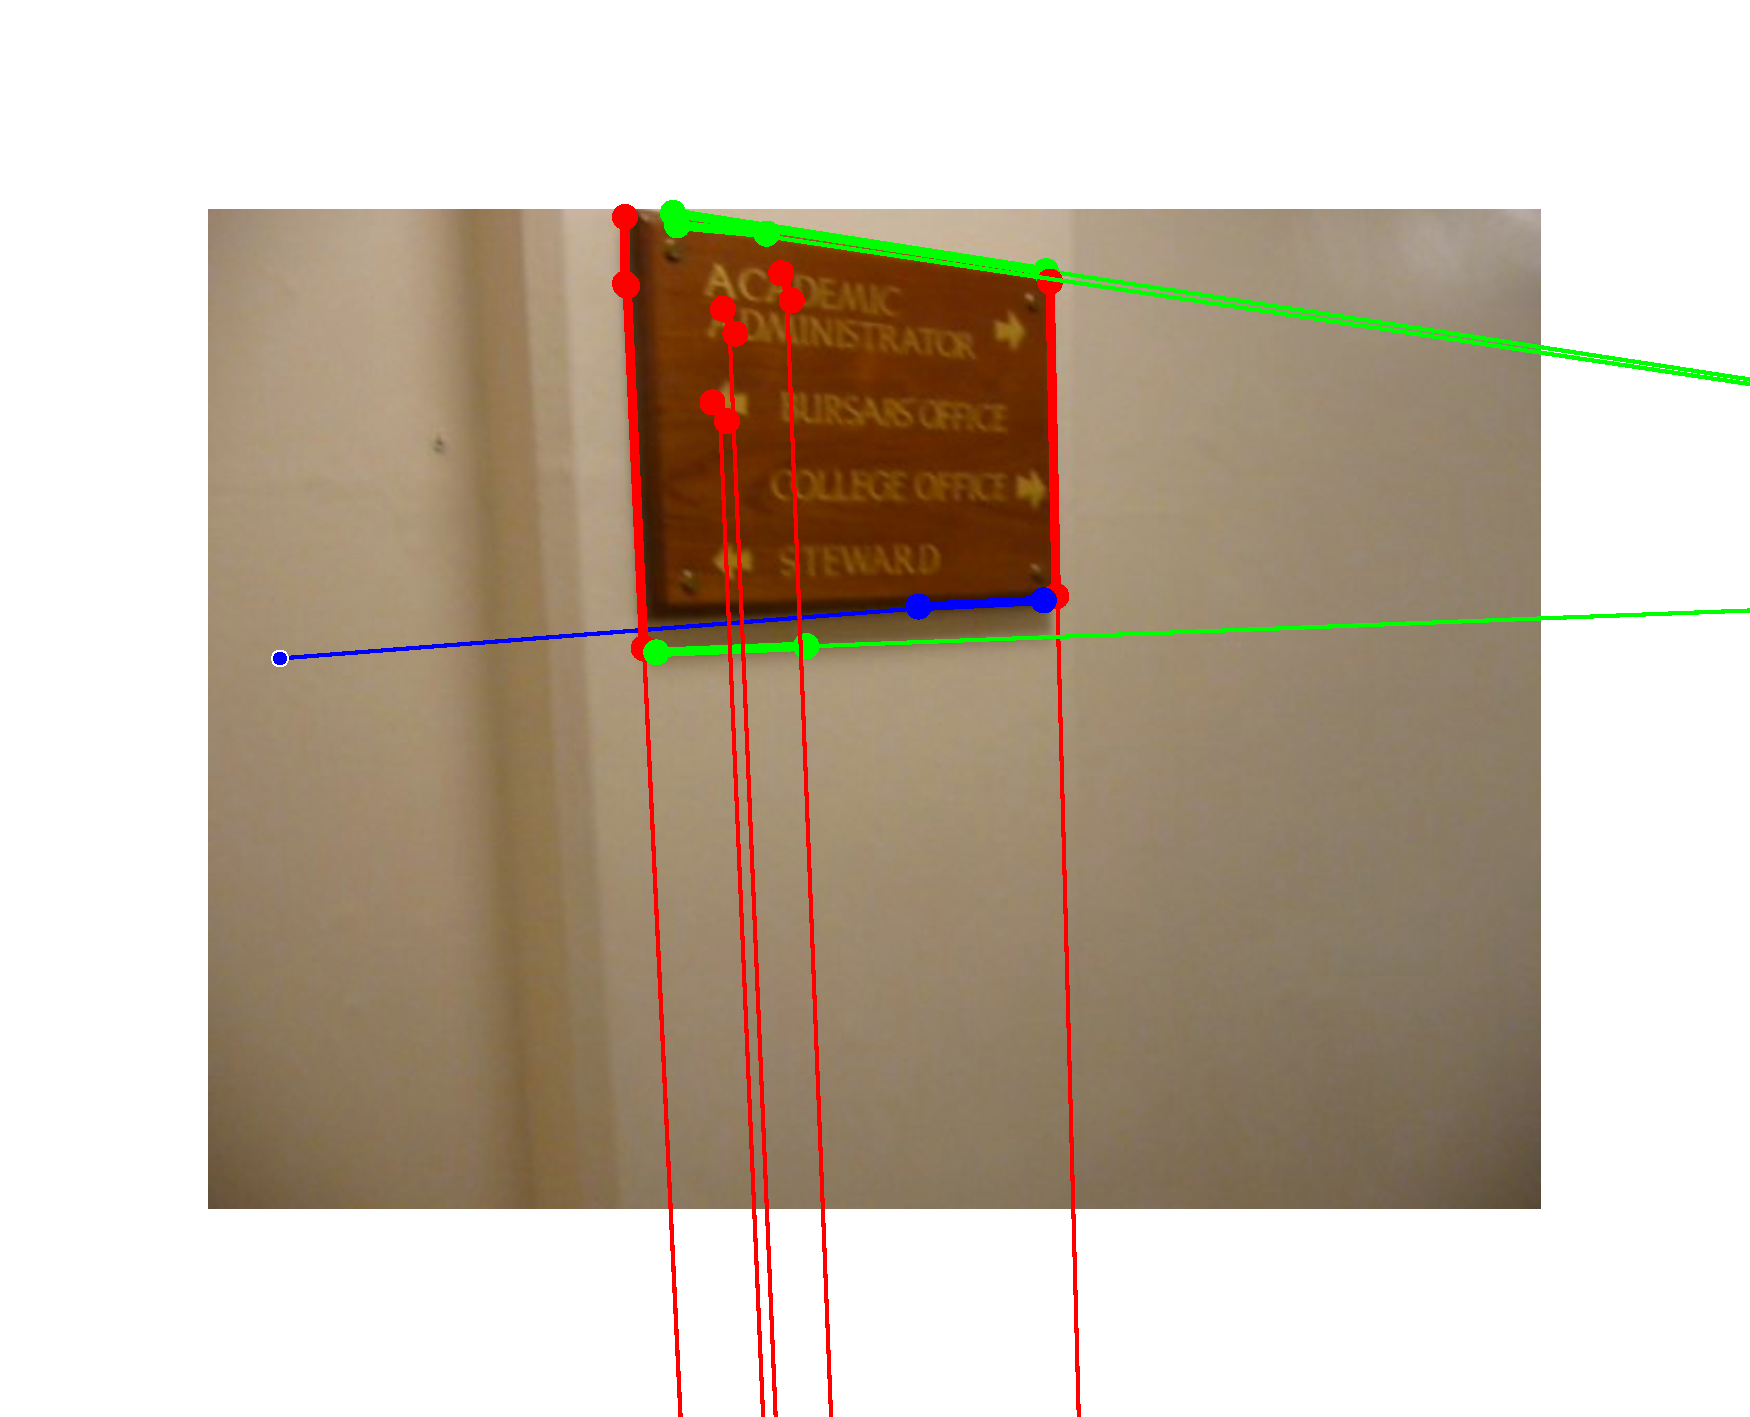
\includegraphics[width=0.46\textwidth]{new_vpt_comparison/exeter_bursary_frame23_vpts_singleimage}
  }\quad
  \subfloat[Geometric (Proposed) Estimate]{
    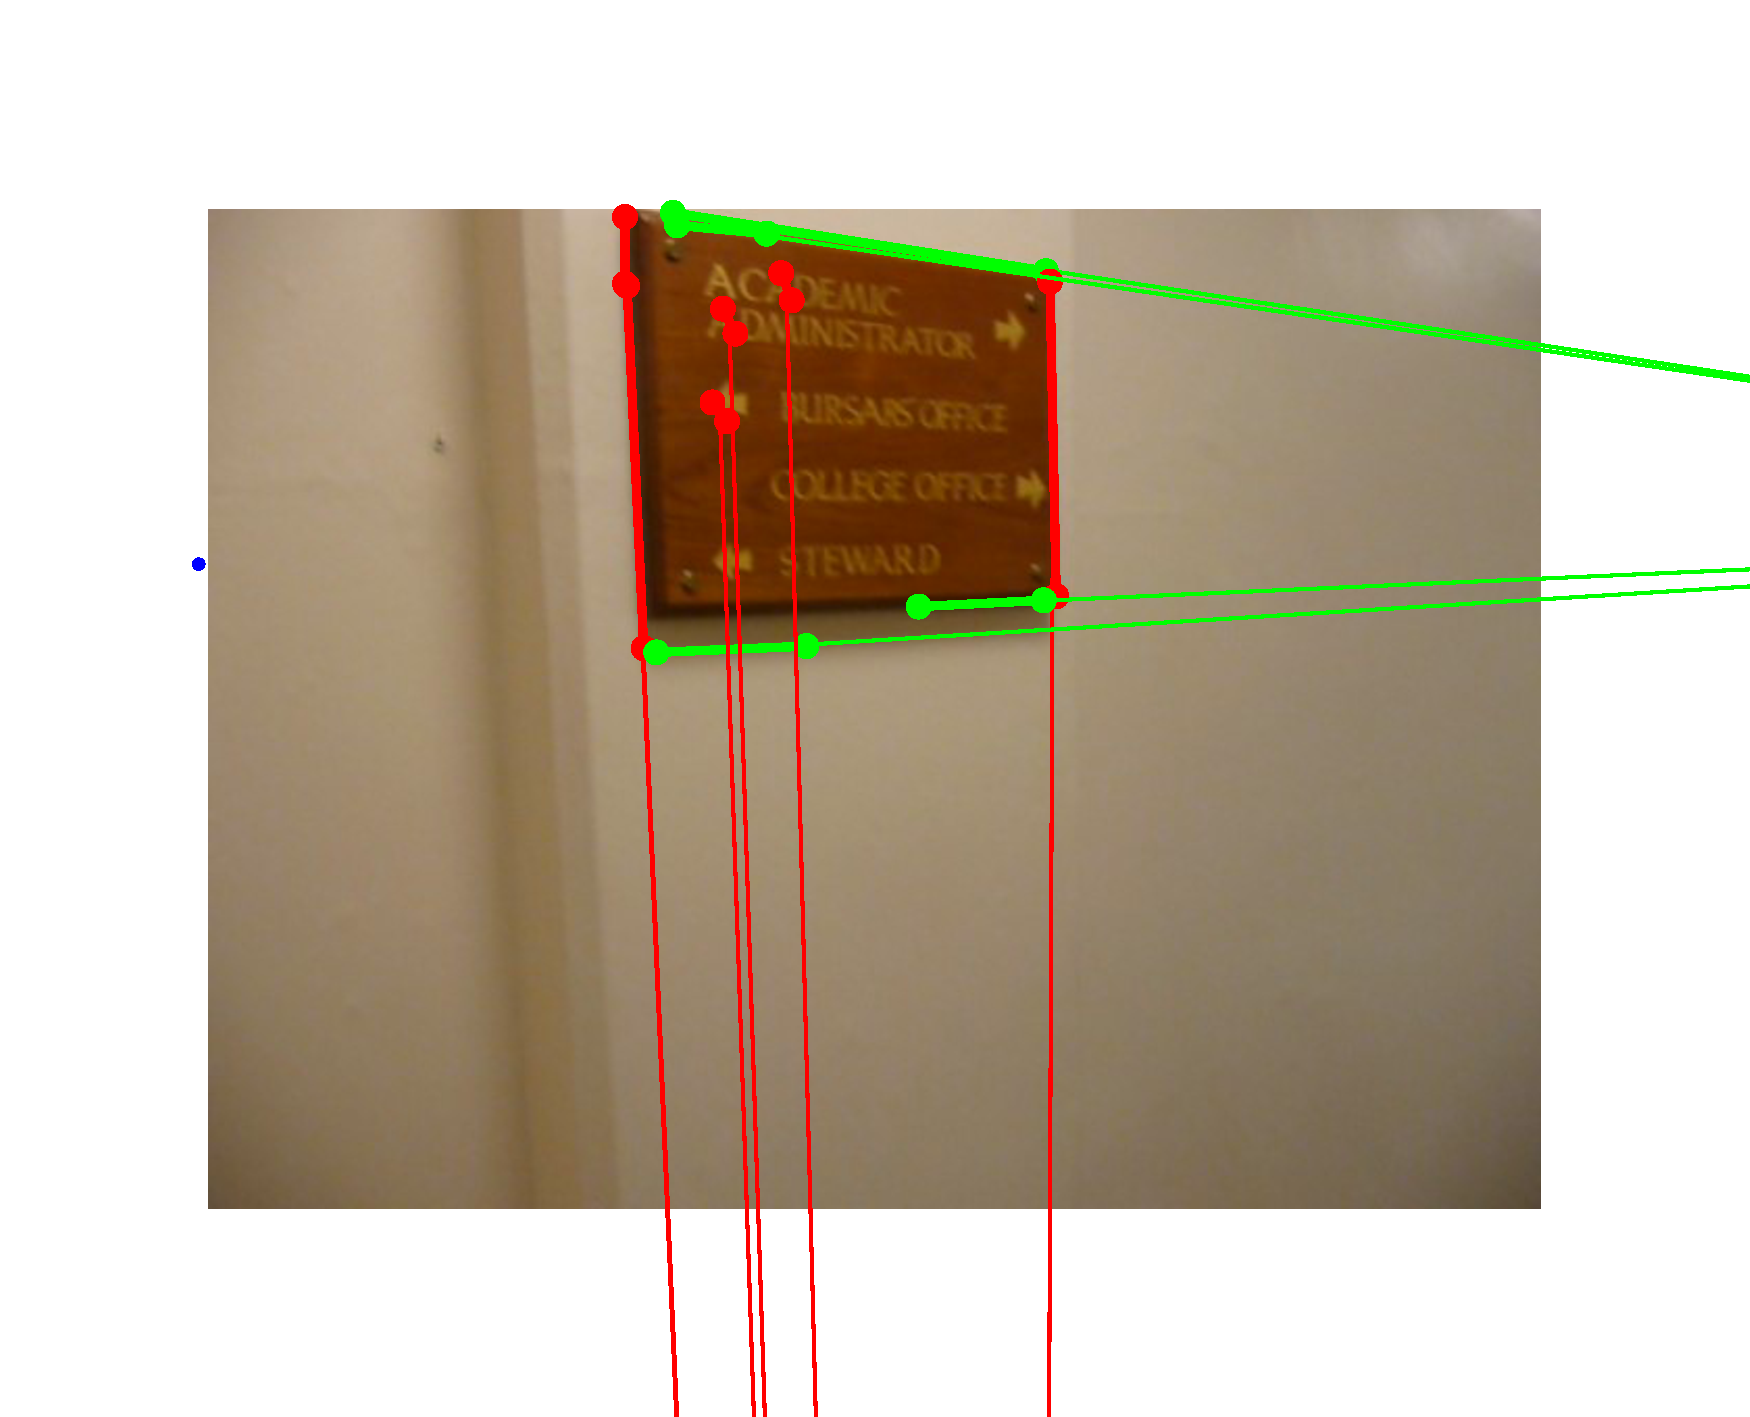
\includegraphics[width=0.46\textwidth]{new_vpt_comparison/exeter_bursary_frame23_vpts_geometric}
  }
  \caption{Comparison of rotation estimation algorithms for an example
    drawn from the ``Bursary'' sequence. Though only one frame is
    shown here, each algorithm other than (c) was provided with 7
    input frames.}
  \label{fig:vpt-example1}
\end{figure}

\begin{figure}[p]
  \centering
  \subfloat[Algebraic Estimate]{
    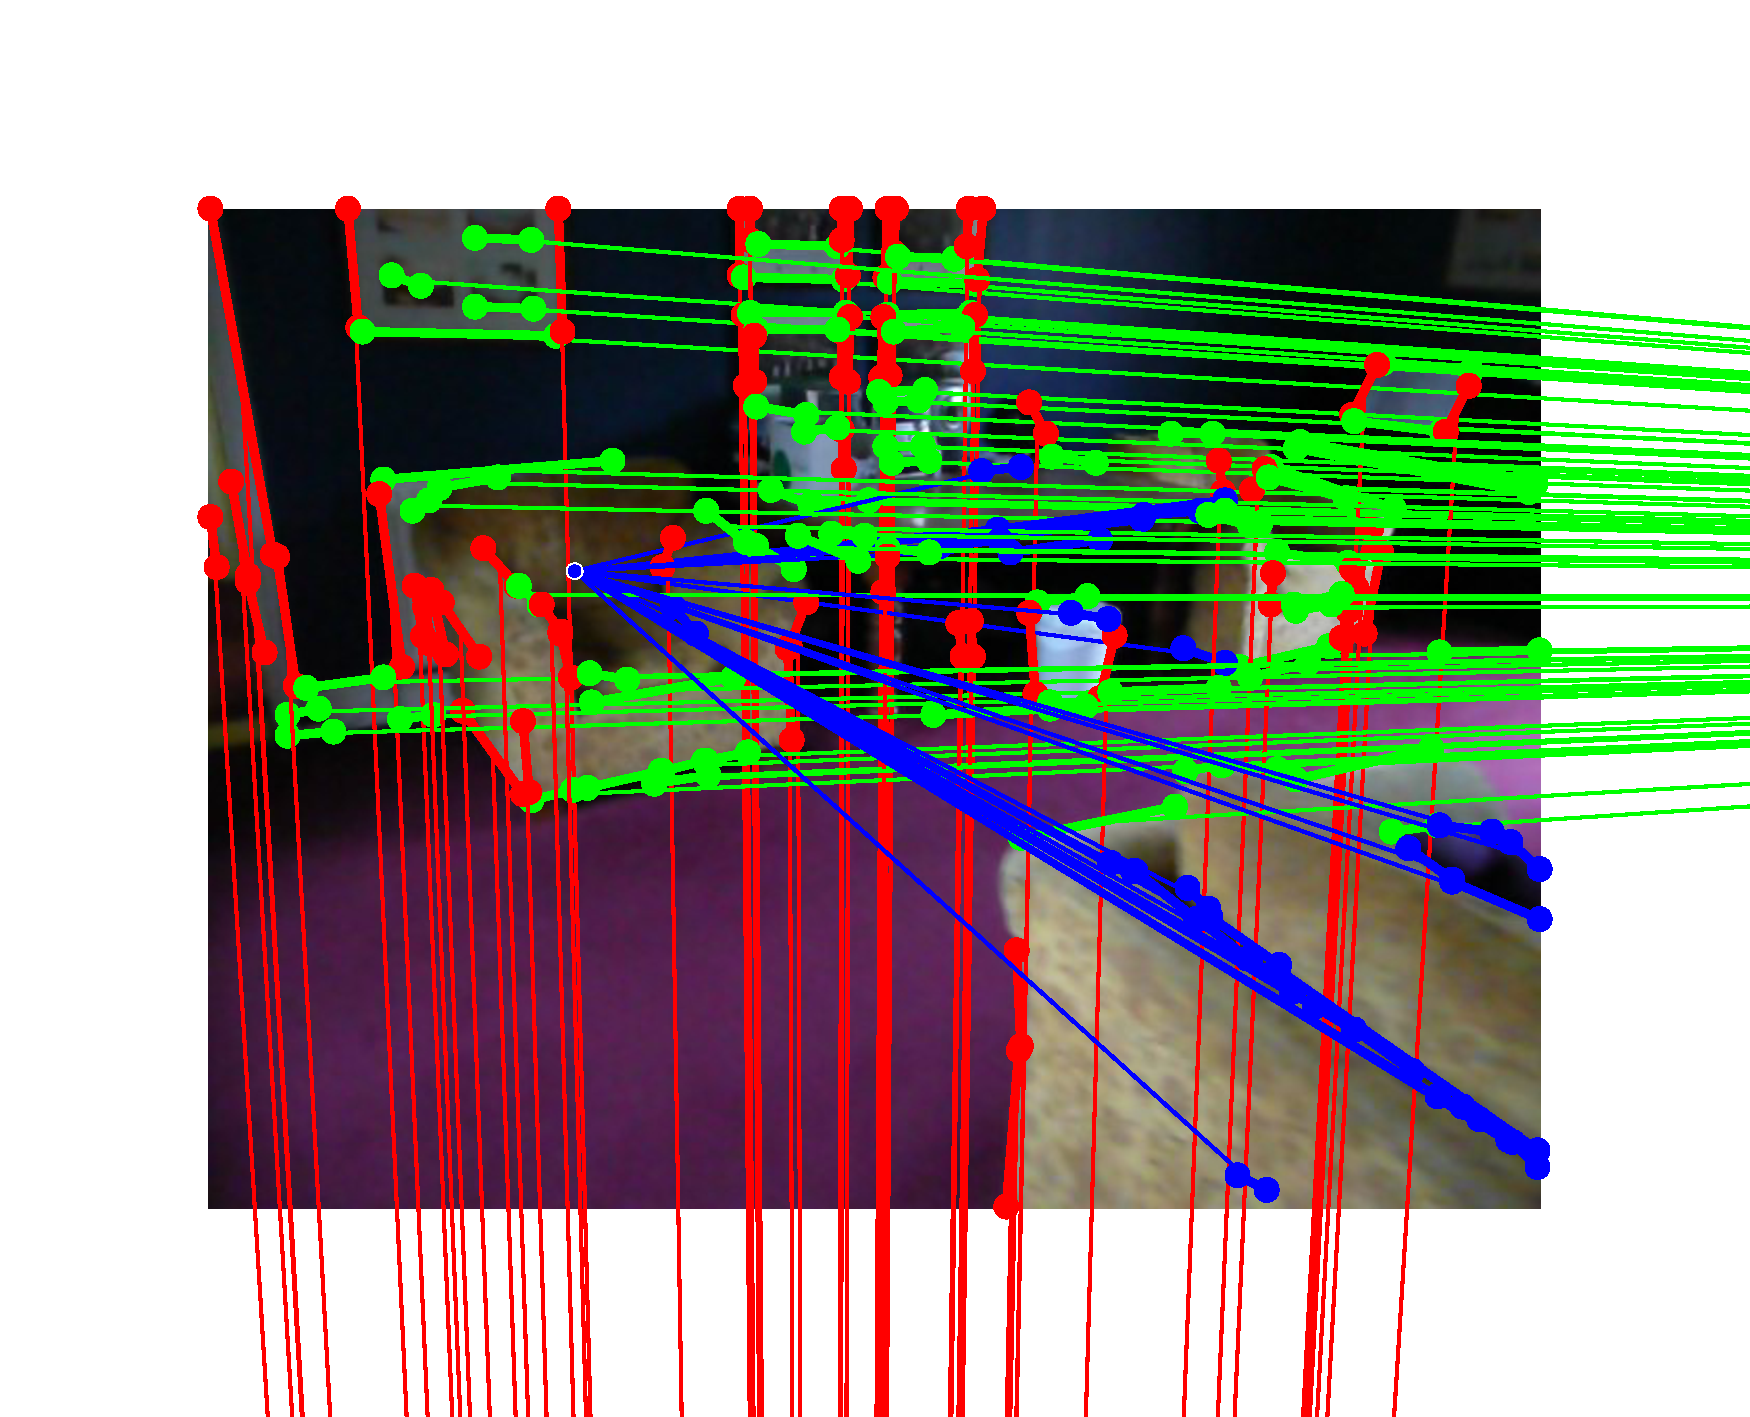
\includegraphics[width=0.46\textwidth]{new_vpt_comparison/exeter_mcr1_frame45_vpts_algebraic}
  }\quad
  \subfloat[Normal--based Estimate]{
    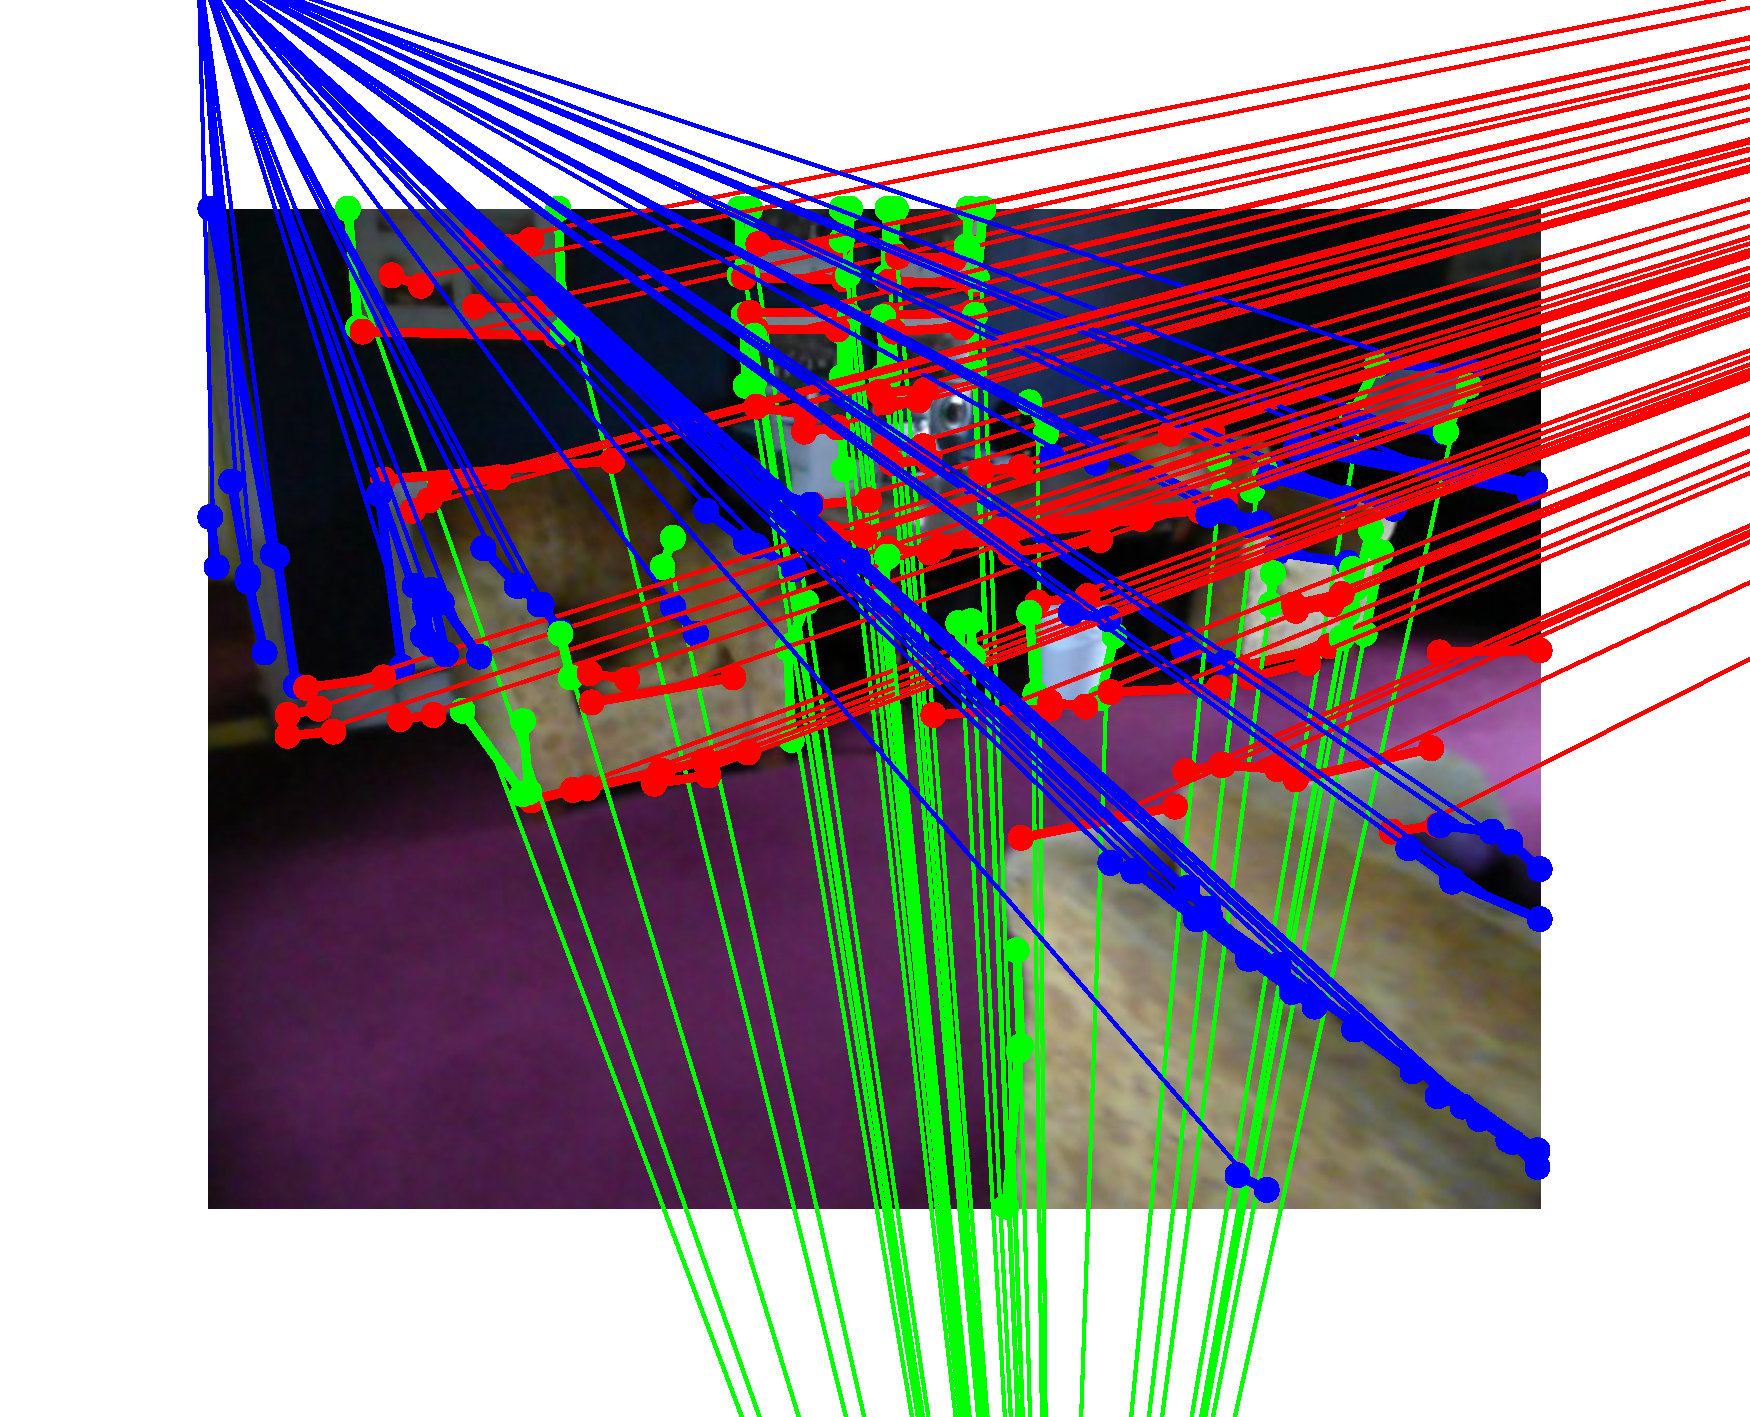
\includegraphics[width=0.46\textwidth]{new_vpt_comparison/exeter_mcr1_frame45_vpts_normals}
  }\\
  \subfloat[Single Image Estimate]{
    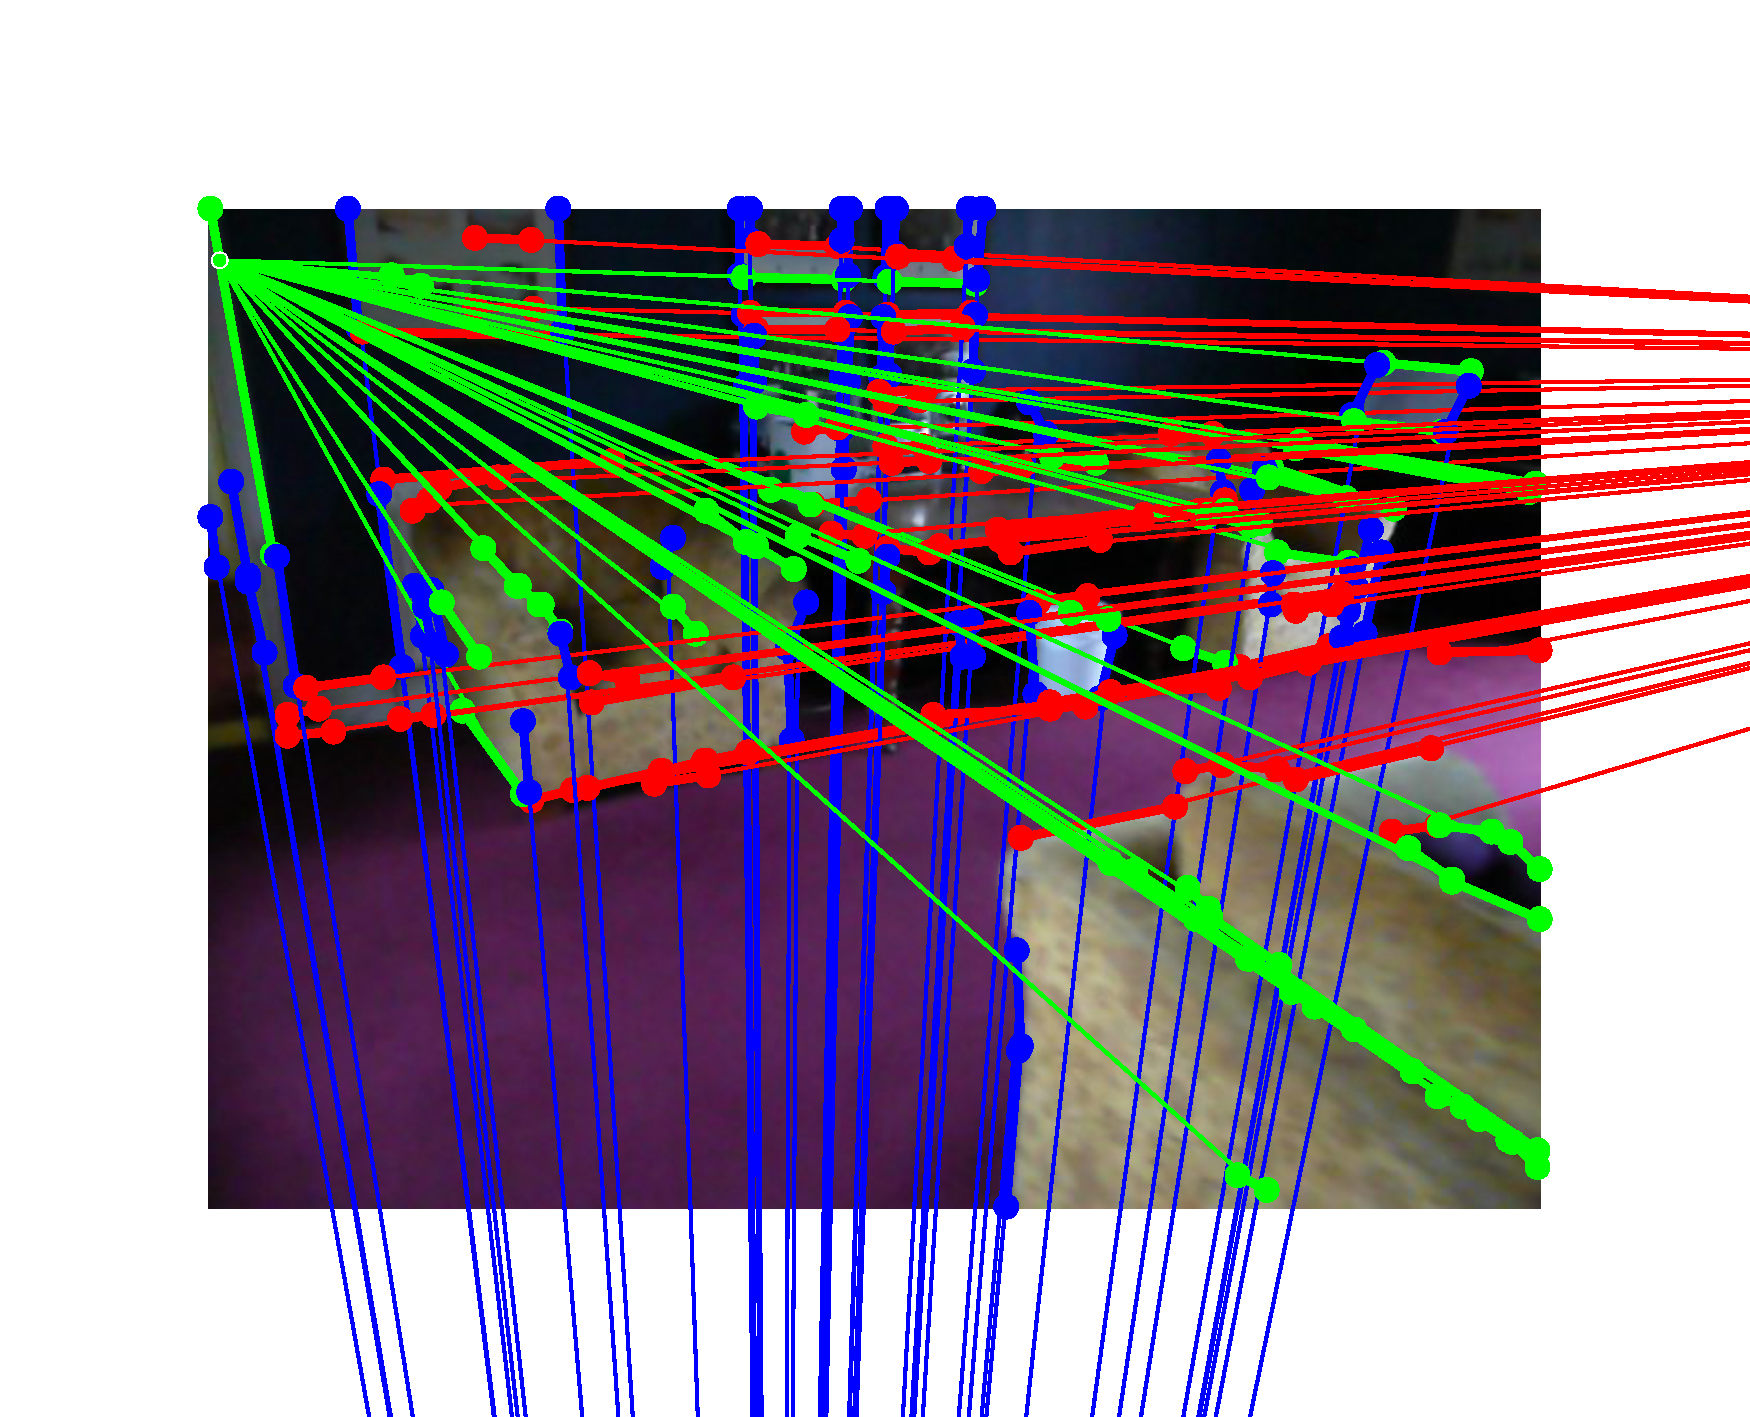
\includegraphics[width=0.46\textwidth]{new_vpt_comparison/exeter_mcr1_frame45_vpts_singleimage}
  }\quad
  \subfloat[Geometric (Proposed) Estimate]{
    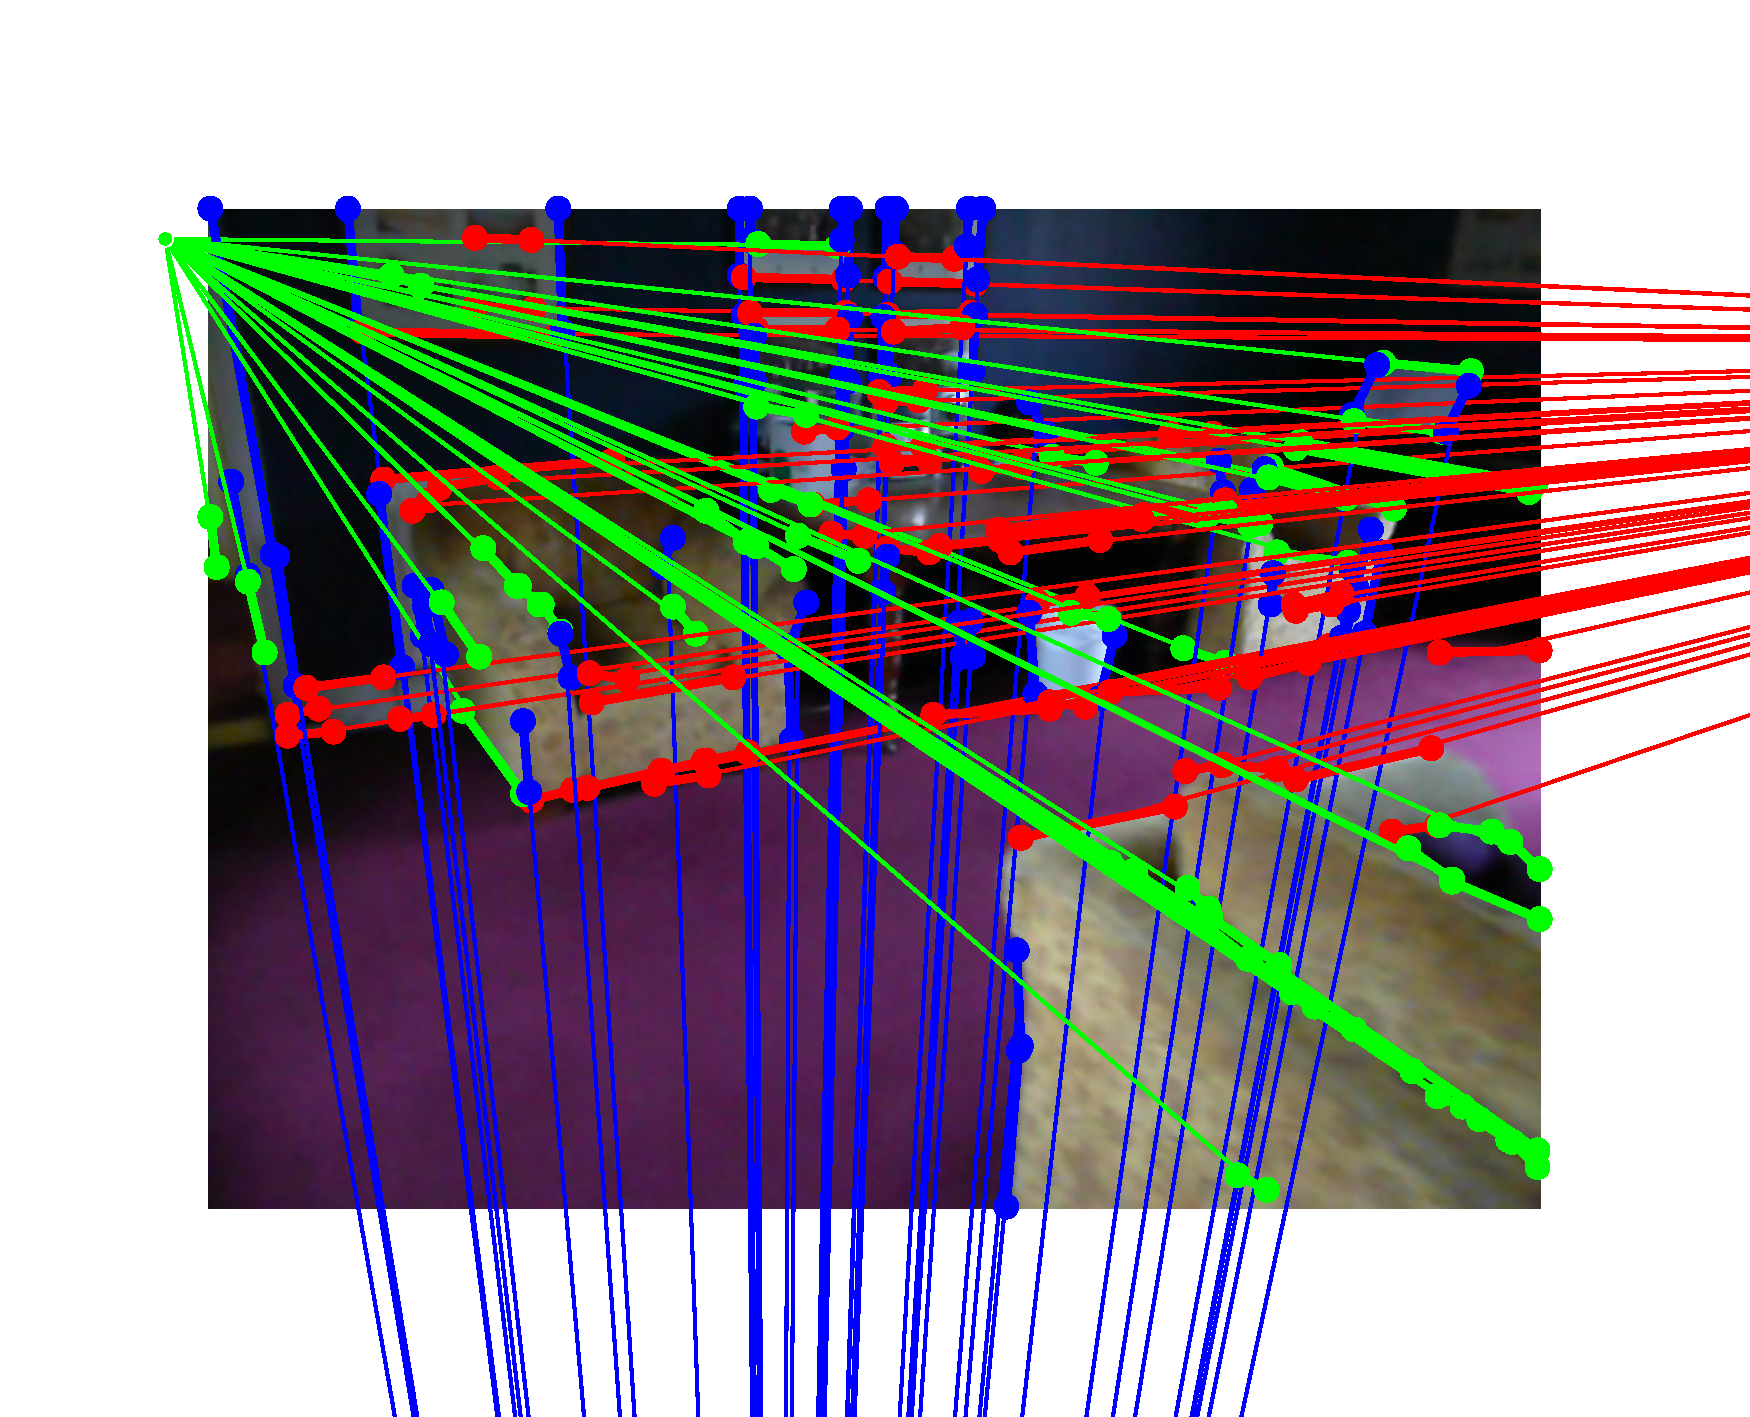
\includegraphics[width=0.46\textwidth]{new_vpt_comparison/exeter_mcr1_frame45_vpts_geometric}
  }
  \caption{Comparison of rotation estimation algorithms for an example
    drawn from the ``MCR'' sequence. Though only one frame is
    shown here, each algorithm other than (c) was provided with 7
    input frames.}
  \label{fig:vpt-example2}
\end{figure}

\begin{figure}[p]
  \centering
  \subfloat[Algebraic Estimate]{
    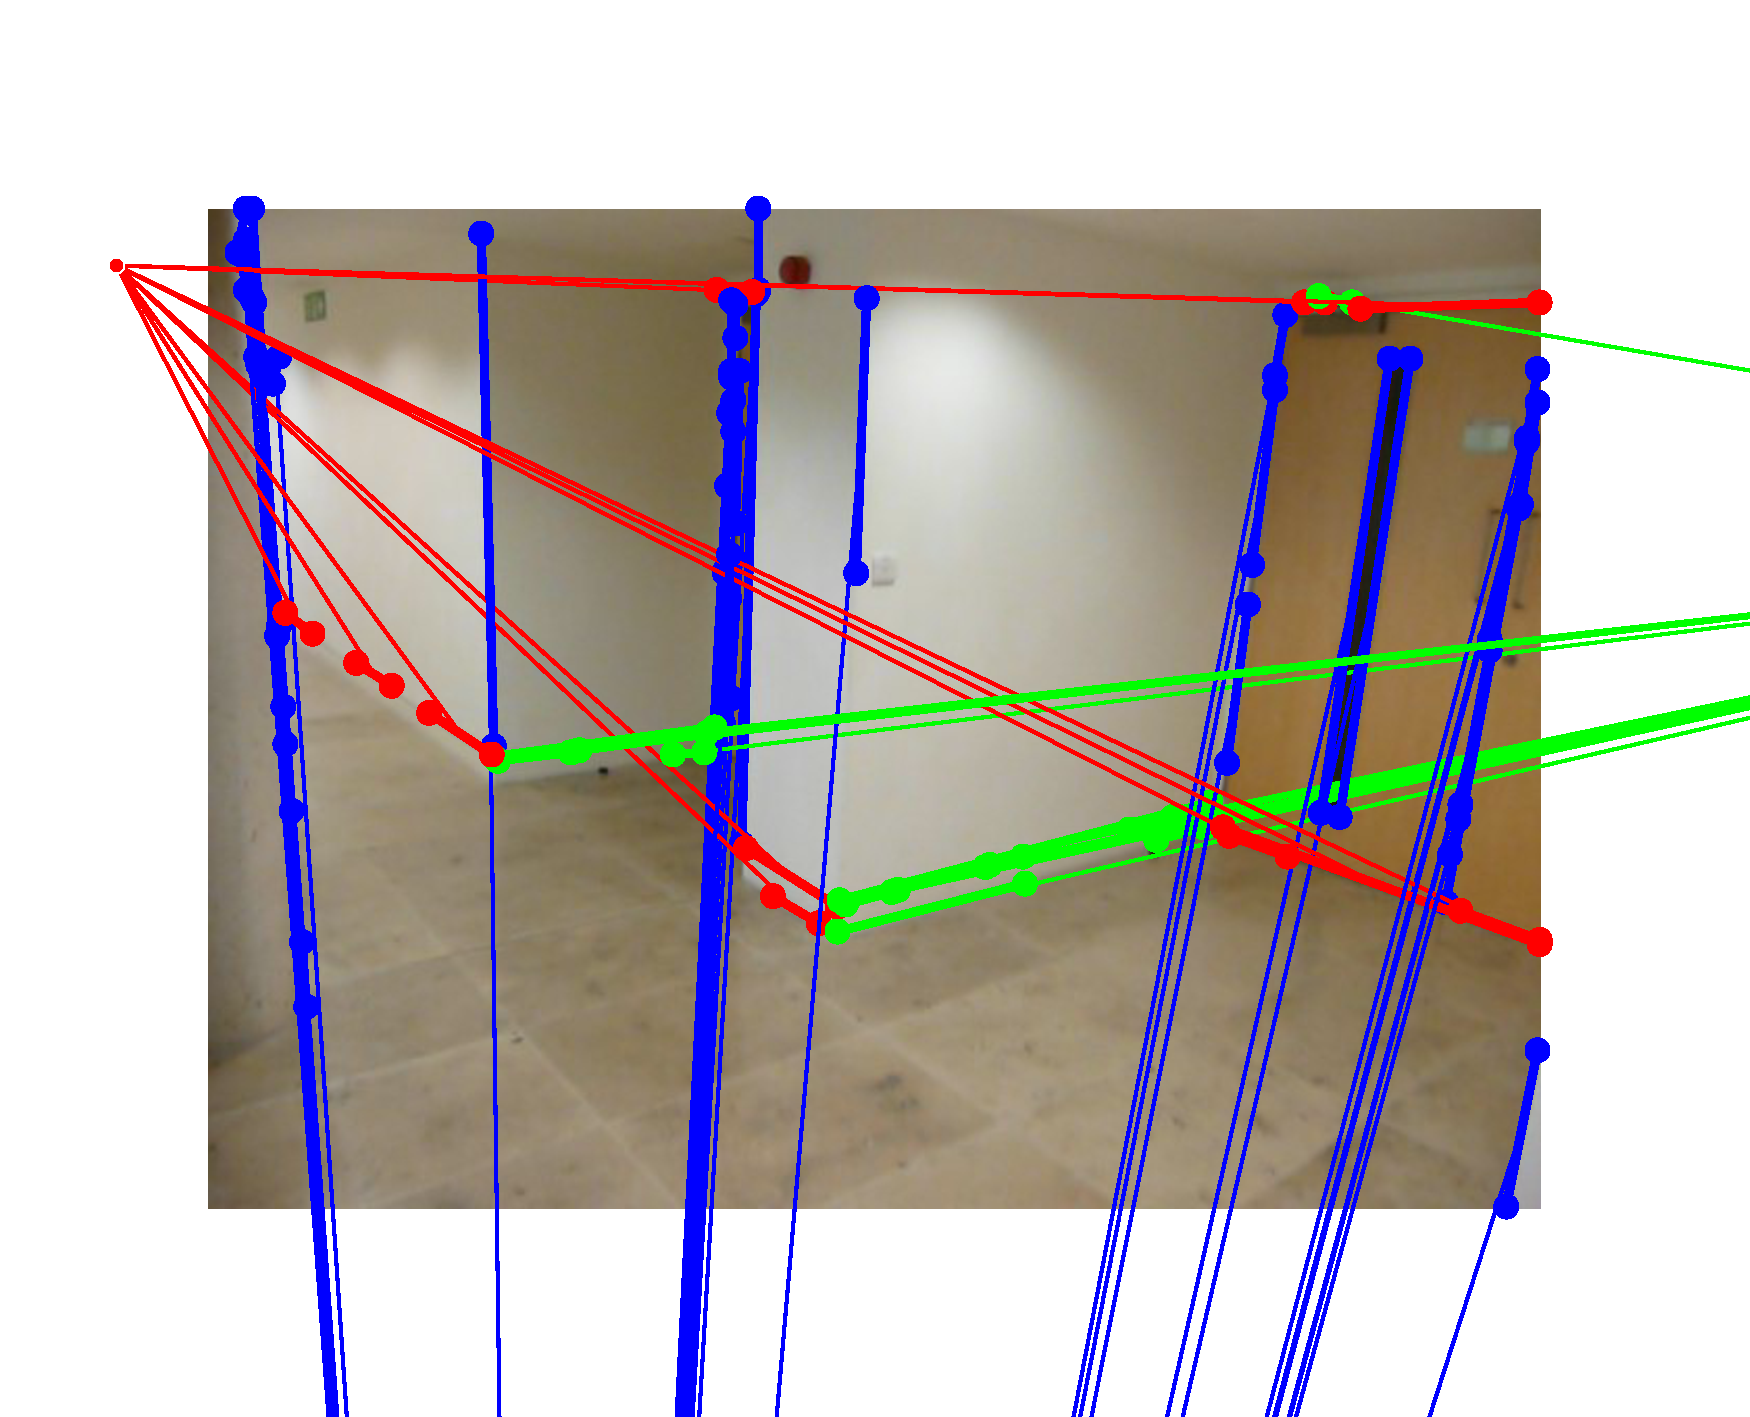
\includegraphics[width=0.46\textwidth]{new_vpt_comparison/lab_ground1_frame21_vpts_algebraic}
  }\quad
  \subfloat[Normal--based Estimate]{
    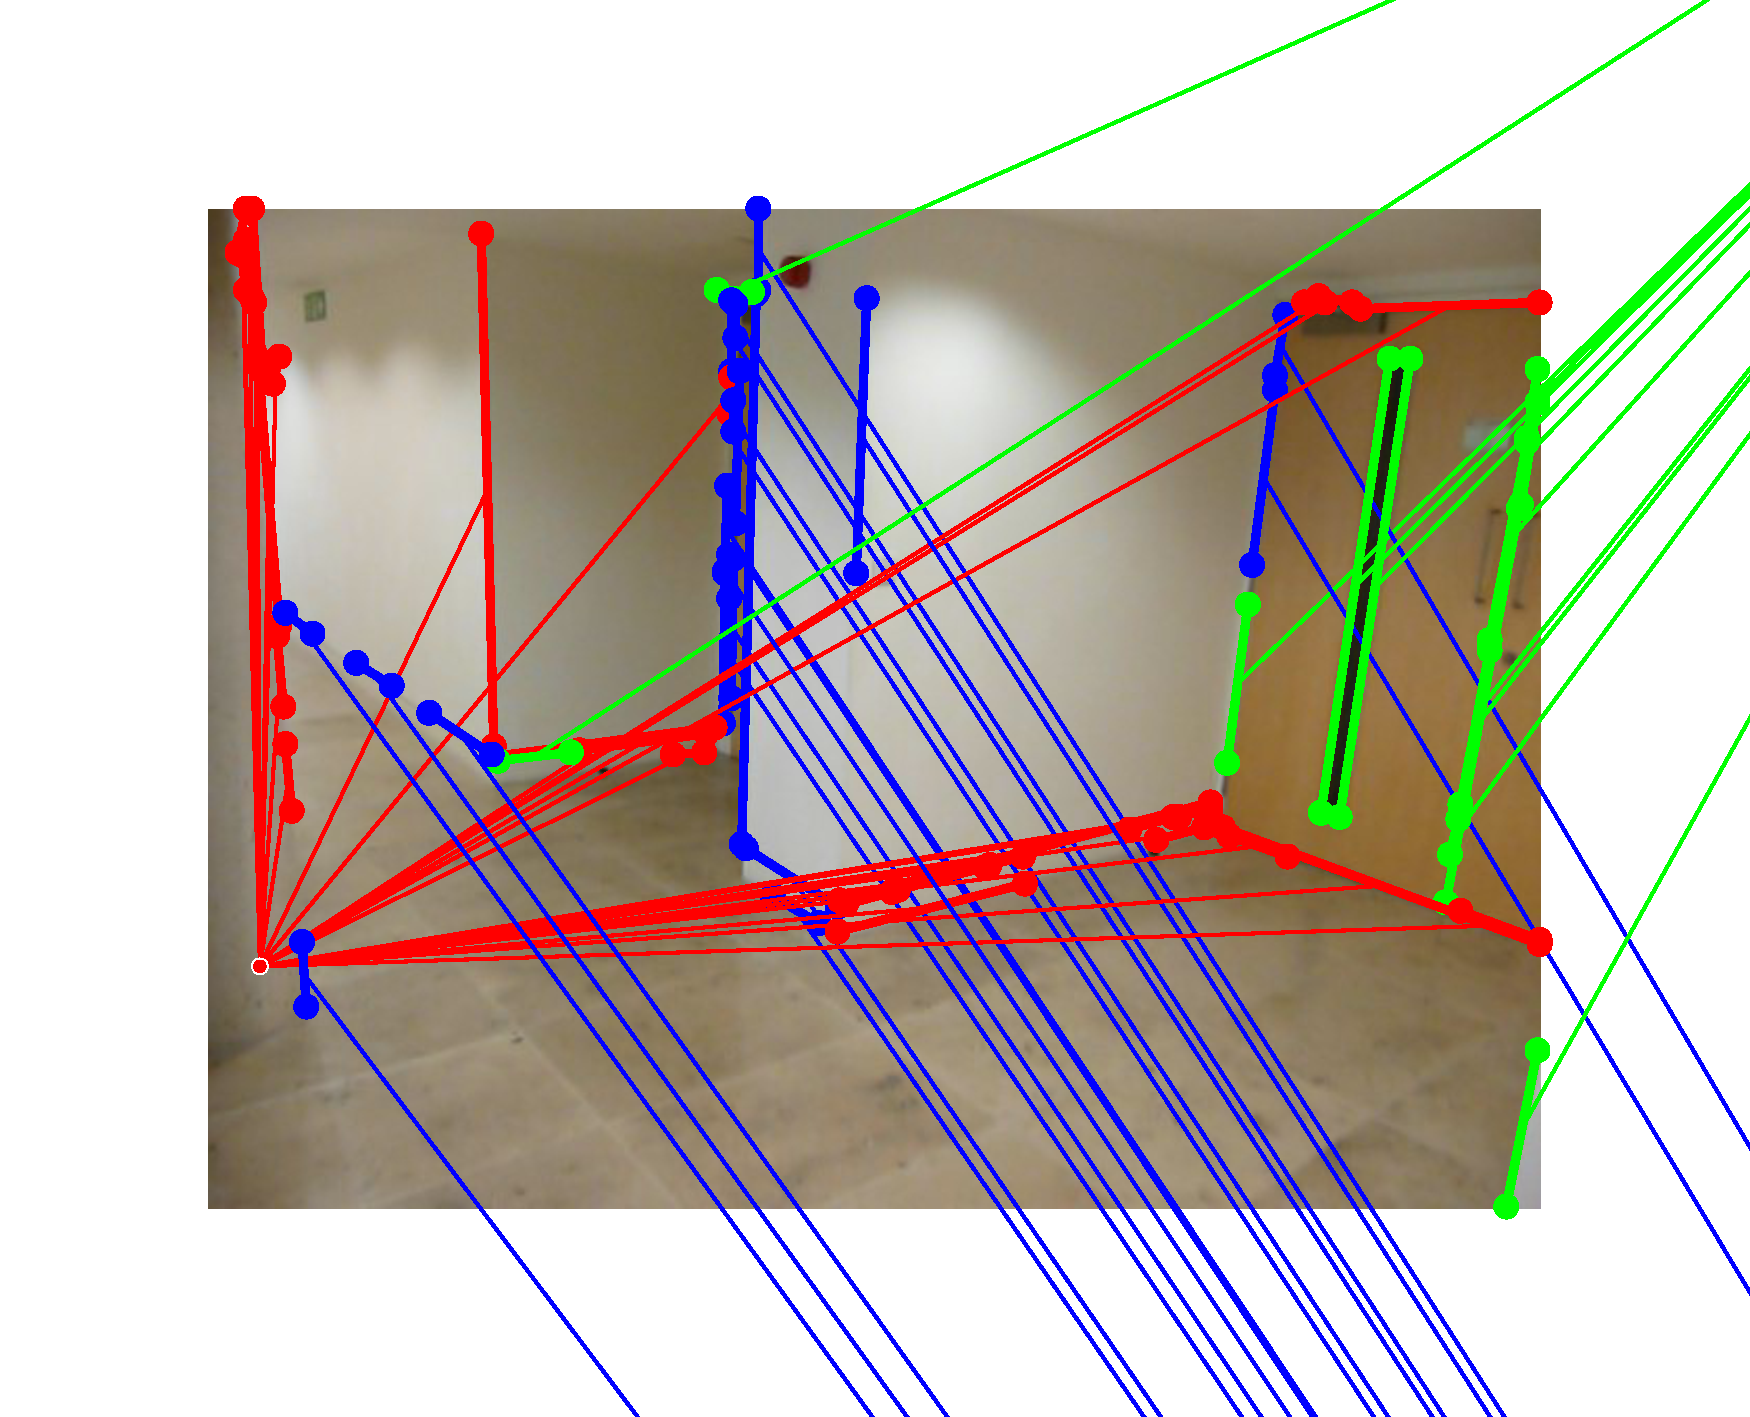
\includegraphics[width=0.46\textwidth]{new_vpt_comparison/lab_ground1_frame21_vpts_normals}
  }\\
  \subfloat[Single Image Estimate]{
    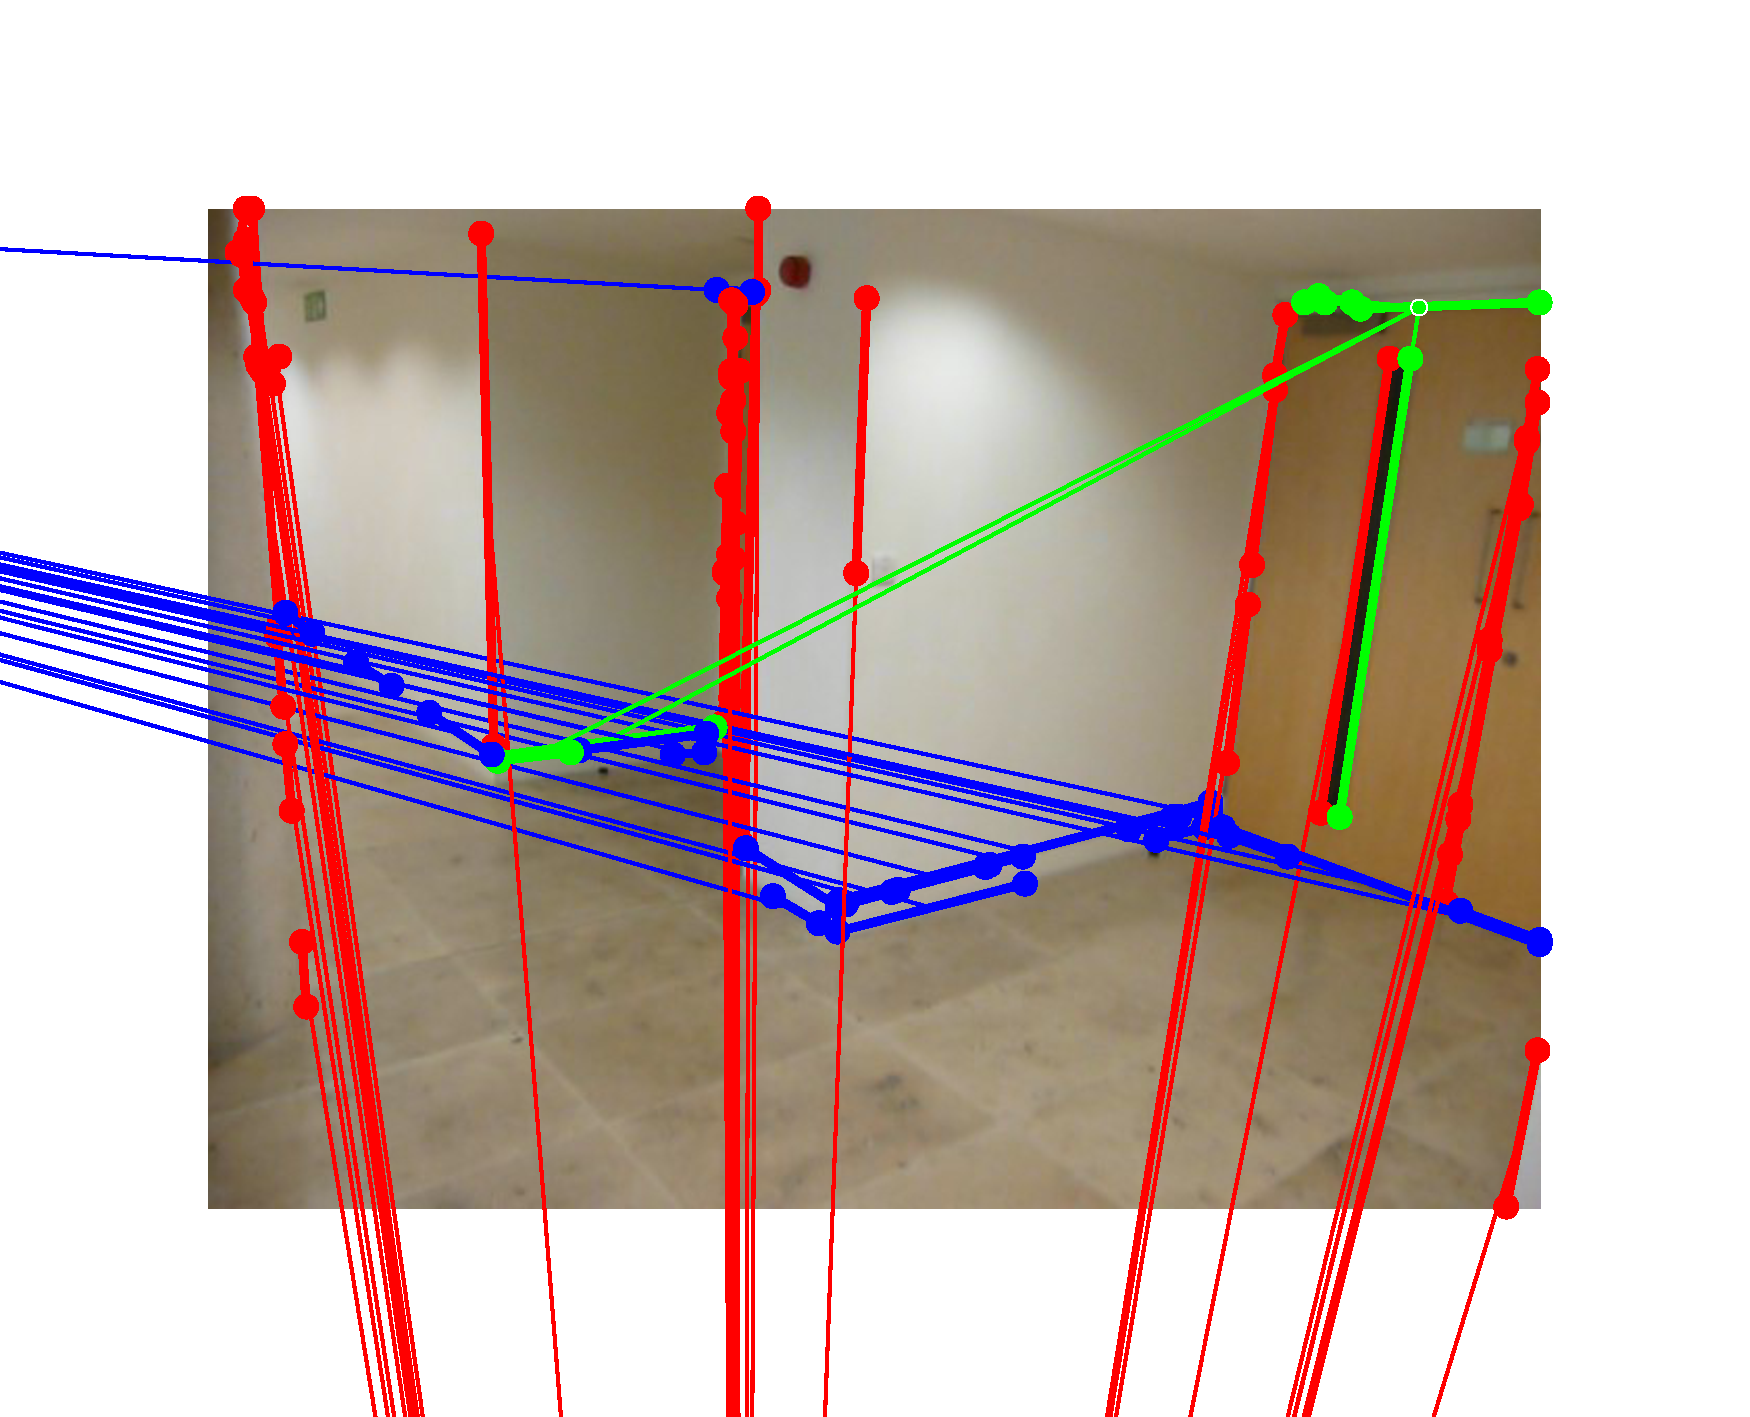
\includegraphics[width=0.46\textwidth]{new_vpt_comparison/lab_ground1_frame21_vpts_singleimage}
  }\quad
  \subfloat[Geometric (Proposed) Estimate]{
    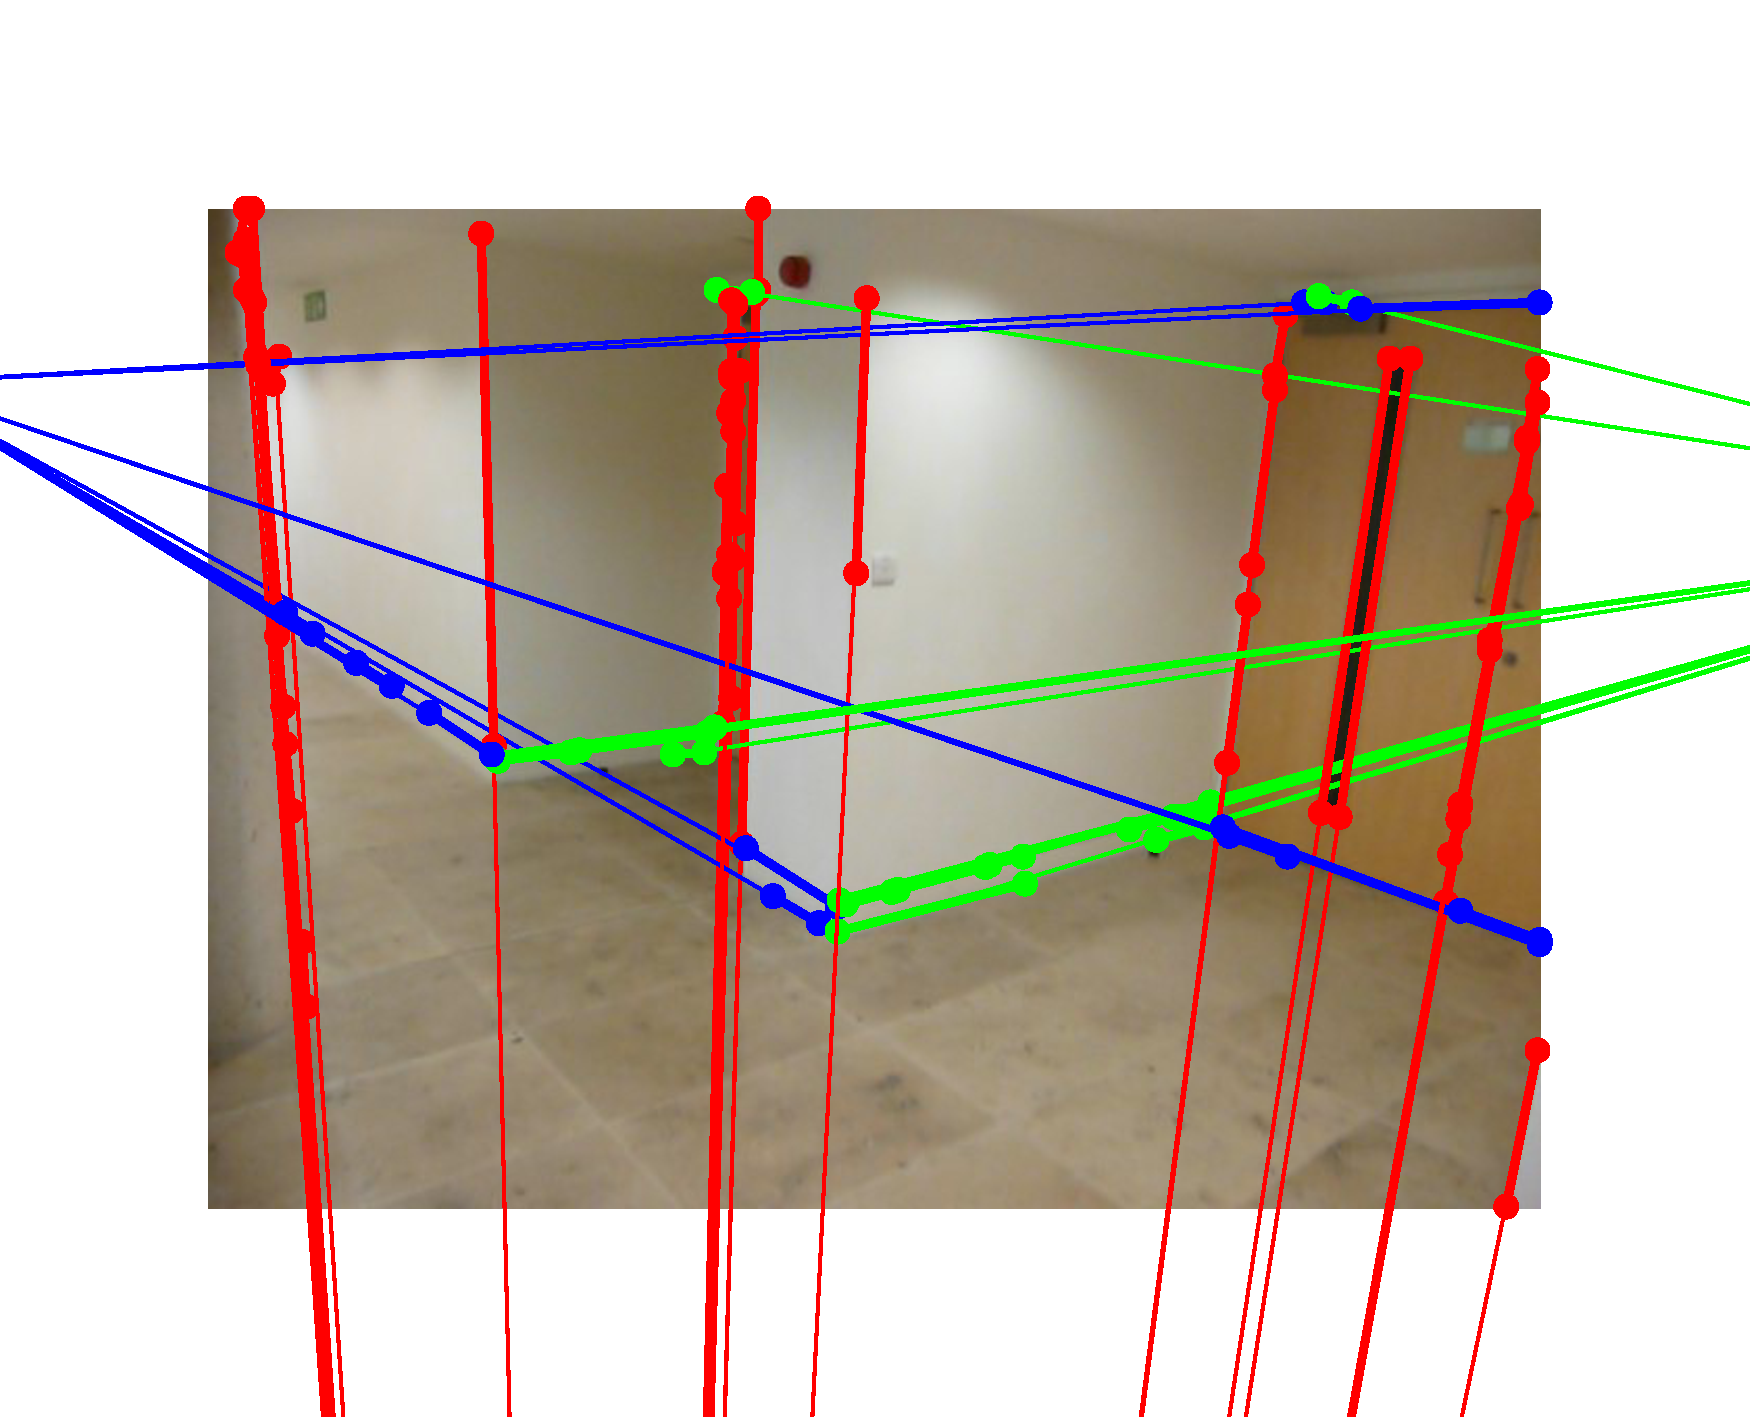
\includegraphics[width=0.46\textwidth]{new_vpt_comparison/lab_ground1_frame21_vpts_geometric}
  }
  \caption{Comparison of rotation estimation algorithms for an example
    drawn from the ``Ground1'' sequence. Though only one frame is
    shown here, each algorithm other than (c) was provided with 7
    input frames.}
  \label{fig:vpt-example3}
\end{figure}

%%%%%%%%%%%%%%%%%%%%%%%%%%%%%%%%%%%%%%%%%%%%%%%%%%%%%%%%%%%%%%%%%%%%%%
\section{Identifying The Vertical Direction}
Of the three dominant directions defined by $\SceneR$, two correspond to
horizontal directions and the third to the vertical direction. The
latter is semantically distinct since it defines the orientation of
the ground and ceiling planes, as well as the direction in which
gravity operates. It is easy to identify the vertical axis since
humans necessarily move over the ground plane when capturing video
sequences, and have limited scope for moving the camera in the
up--down direction. We therefore set the vertical axis to that over
which camera positions range the least. Having identified $\SceneR$ there
are only three possible choices, and we found this heuristic to work
correctly in all of our evaluation sequences.

%%%%%%%%%%%%%%%%%%%%%%%%%%%%%%%%%%%%%%%%%%%%%%%%%%%%%%%%%%%%%%%%%%%%%%
\section{Identifying The Floor And Ceiling Planes}
\label{sect:fcmap}

\begin{figure}[tb]
  \centering
  \subfloat[]{
    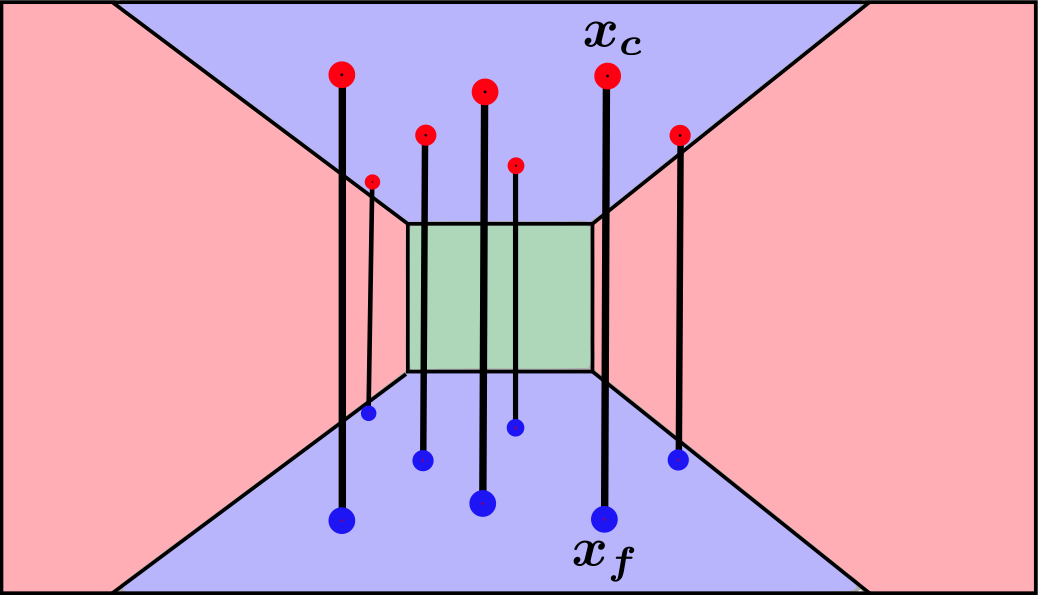
\includegraphics[width=0.4\textwidth]{manhattan-homology}
  }\quad
  \subfloat[]{
    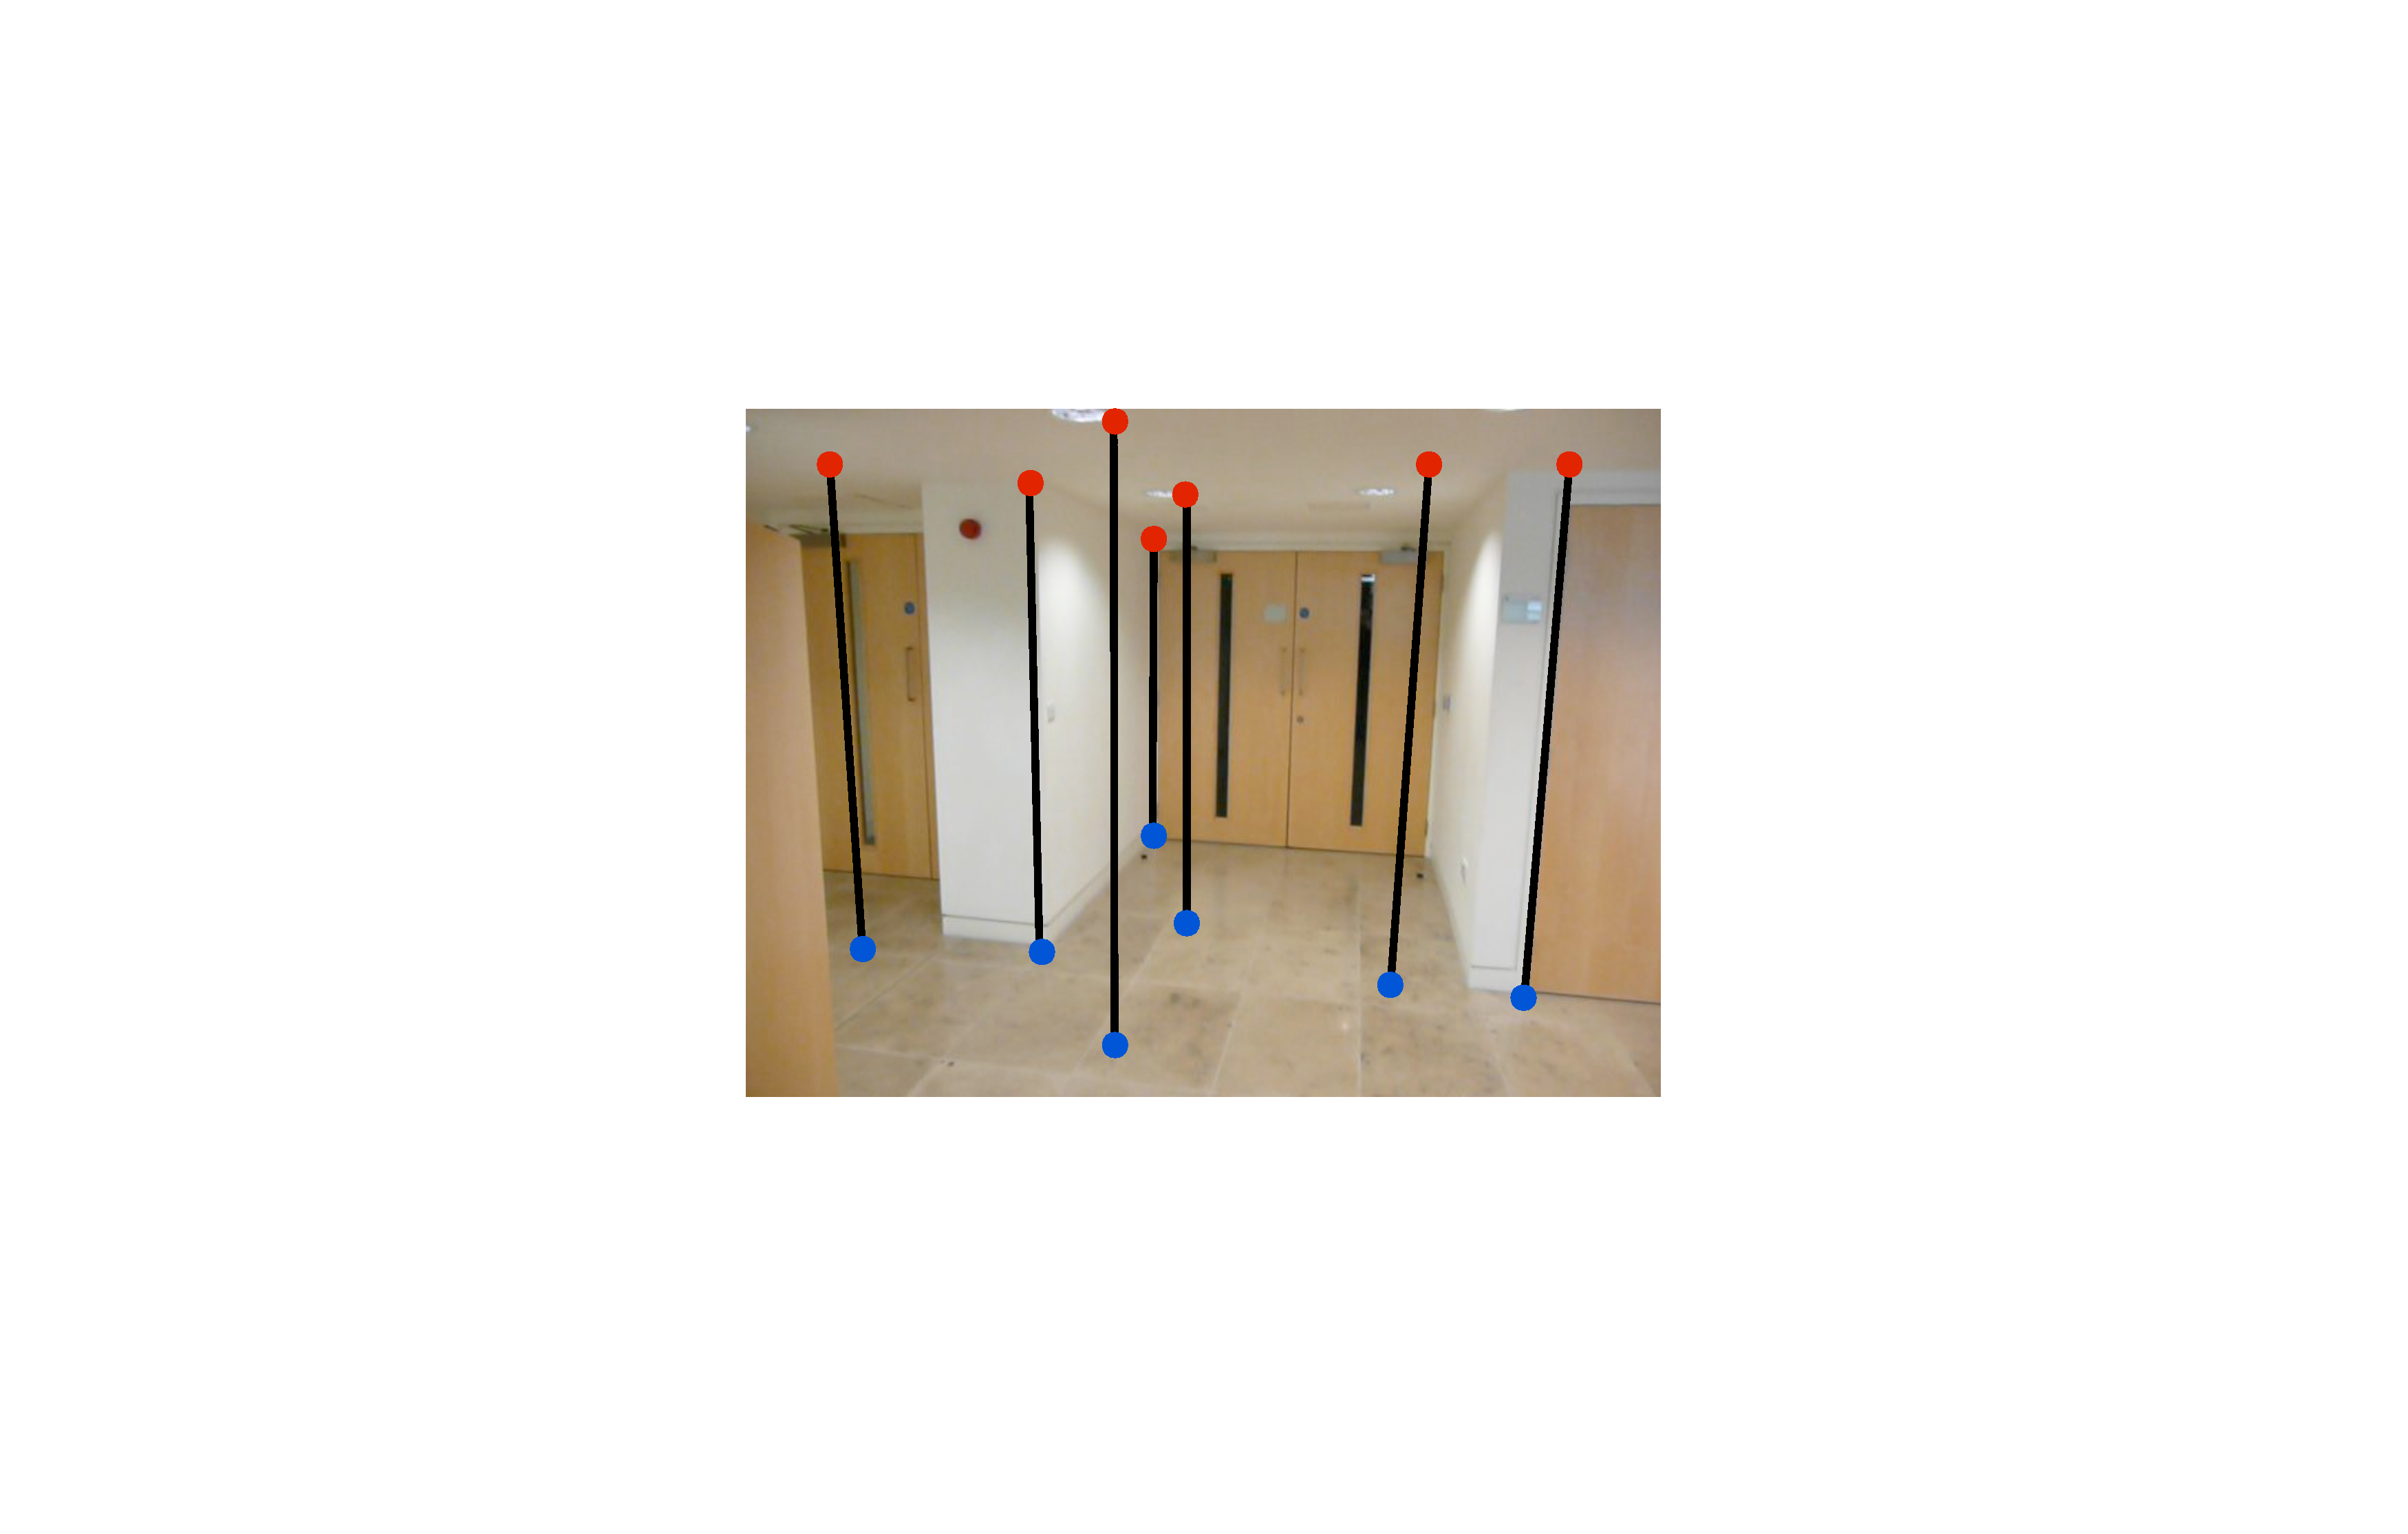
\includegraphics[width=0.4\textwidth]{manhattan-homology-realworld}
  }
  \caption{\changedsinceviva{The mapping $\Hcf$ transfers points between the ceiling and
    floor in the image domain. $\Hcf$ is a planar homology.}}
  \label{fig:fcmap}
\end{figure}

An indoor Manhattan scene has exactly one floor and one ceiling plane,
both with normal $\vvpt$. It will be useful in the following chapters
to have available the mapping $\Hcf$ between the image locations of
ceiling points the floor points that are vertically below them (see
\figref{fcmap}). $\Hcf$ is a planar homology with axis
$\horizon=\lvpt\cross\rvpt$ and vertex $\vvpt$ \cite{Criminisi01} and
can be recovered given the image location of any pair of corresponding
floor/ceiling points $(\FloorPt,\CeilPt)$ as
\begin{equation}
  \Hcf = I + \mu\frac{\vvpt\horizon^T}{\vvpt \cdot \horizon} ~,
\end{equation}
where
\begin{equation}
  \mu = \bigl\langle\vvpt,\CeilPt,\FloorPt,
  \CeilPt\times\FloorPt\times\horizon\bigr\rangle
\end{equation}
is the characteristic cross ratio of $\Hcf$. Although we do not have
\textit{a priori} any such pair $(\FloorPt,\CeilPt)$, we can recover
$\Hcf$ using the following sampling algorithm. First we identify edges
in the image using one of the many available edge detection
algorithms. Next we sample one edge pixel $\vect{\hat{x}_c}$ from the
region above the horizon, then we sample a second point
$\vect{\hat{x}_f}$ collinear with the first and $\vvpt$ from the
region below the horizon. We then compute a hypothesis for $\Hcfhat$
as described above, and then assign a score by counting the number of
edge pixels that $\Hcfhat$ maps onto other edge pixels. After
repeating this for a fixed number of iterations we return the
hypothesis with greatest score.

Many images contain either no view of the floor or no view of the
ceiling. In such cases $\Hcf$ is unimportant since there are no
corresponding points in the image. If the best $\Hcf$ output from the
sampling process has a score below a threshold $k_t$ then we set $\mu$
to a large value that will transfer all pixels outside the image
bounds. $\Hcf$ will then have no impact on the estimated model.

In the context of multiple views we resolve scale by identifying
$\ScaleParam$ with either the maximum or minimum $z$ component of any
point in the point cloud reconstructed by structure--from--motion.

%% \subsection{Identifying the floor and ceiling planes.}
%% An indoor Manhattan scene has exactly one floor and one ceiling plane,
%% both with normal direction $\vvpt$. It will be useful in the following
%% sections to have available the mapping $\Hcf$ between the image
%% locations of ceiling points and the image locations of the floor
%% points that are vertically below them (see \figref{fcmap}). $\Hcf$ is
%% a planar homology with axis $\vect{h}=\lvpt\times\rvpt$ and vertex
%% $\vvpt$ \cite{Criminisi01} and can be recovered given the image
%% location of any pair of corresponding floor/ceiling points
%% $(\vect{x_f},\vect{x_c})$ as
%% \begin{equation}
%%   \Hcf = I + \mu\frac{\vvpt\vect{h}^T}{\vvpt \cdot \vect{h}} ~,
%% \end{equation}
%% where $\mu = \langle\vvpt,\vect{x_c},\vect{x_f},
%% \vect{x_c}\times\vect{x_f}\times\vect{h}\rangle$ is the characteristic cross
%% ratio of $\Hcf$.

%% Although we do not have \textit{a priori} any such pair
%% $(\vect{x_f},\vect{x_c})$, we can recover $\Hcf$ using the following
%% RANSAC algorithm. First, we sample one point $\vect{\hat{x}_c}$ from
%% the region above the horizon in the Canny edge map, then we sample a
%% second point $\vect{\hat{x}_f}$ collinear with the first and
%% $\vvpt$ from the region below the horizon. We compute the
%% hypothesis map $\Hcfhat$ as described above, which we then score by
%% the number of edge pixels that $\Hcfhat$ maps onto other edge pixels
%% (according to the Canny edge map). After repeating this for a fixed
%% number of iterations we return the hypothesis with greatest score.

%% Many images contain either no view of the floor or no view of the
%% ceiling. In such cases $\Hcf$ is unimportant since there are no
%% corresponding points in the image. If the best $\Hcf$ output from the
%% RANSAC process has a score below a threshold $k_t$ then we set $\mu$
%% to a large value that will transfer all pixels outside the image
%% bounds. $\Hcf$ will then have no impact on the estimated model.

\section{Extension: Relaxing The Manhattan World Assumption}
The strong Manhattan assumption states that any pair of surfaces of
interest are either parallel or orthogonal to one another. One common
deviation from this is scenes with walls that are orthogonal to the
floor and ceiling but not to one another. We define the weak Manhattan
assumption as ``the environment consists of a horizontal ground plane
and corresponding ceiling plane, and a set of vertical wall segments
extending continuously between them.'' Weakly Manhattan environments
contain much of the regularity of strongly Manhattan environments, and
here we discuss how to extending the approach taken in chapter to such
scenes. We have not implemented this approach; we discuss these ideas
as inspiration for future work.

We can deal with the weak Manhattan assumption as follows. First, we
run the EM algorithm described above to obtain $\SceneR$. Next, for
each line $\LineSeg_j$ marked as spurious by the EM algorithm we find
its intersection with the horizon,
\begin{equation}
  \vect{u}_j = \SceneR^{-T} R_i^{-T} \LineSeg_j \times \ez ~,
\end{equation}
which would be its vanishing point if it were horizontal in the
world. Vertical surfaces of a given orientation will generate
identical $\vect{u}_j$ (modulo measurement error), so we may identify
additional vertical orientations by clustering the intersections
$\{\vect{u}_j\}$. This should be possible even with few such
intersections, since the fact that all intersections are on the
horizon reduces this to a one--dimensional estimation problem.

%% We adopt a voting algorithm in which we parametrise
%% $\vect{u}_j$ in terms of the angle $\theta_j$ about the $z$ axis
%% \begin{equation}
%%   \theta_{j} = \mbox{atan}
%%   ({\ey}^T\vect{u}_j,~ {\ex}^T\vect{u}_j) ~.
%% \end{equation}
%% We accumulate the $\theta_j$ into histogram bins and identify any
%% local maxima $\theta_i^*$ above a threshold $k$. Each $\theta_i^*$
%% represents a cluster of line segments corresponding to an additional
%% vertical orientation. Finally, we re--estimate the vanishing point for
%% each cluster by minimising the likelihood \eqref{line-lik} via
%% least--squares.

\section{Conclusion}

We have proposed a principled approach to discovering the dominant
Manhattan directions given multiple calibrated views. Our likelihoods
are derived from a well--defined model of image generation, and we
solve inference as a single optimisation. Our work is strongly
influenced by the literature on vanishing point detection and our
approach parallels ideas previously proposed in the single--view
context. Our contribution is a principled way to incorporate multiple
calibrated views into a single optimisation, and an empirical
demonstration that doing so significantly out--performs both
single--view vanishing point estimation and surface--normal--based
estimators.
